%%%%%%%%%%%%%%%%%%%%%%%%%%%%%%%%%%%%%%%%%%%%%%%%%%%%%%%%%%%%%%%%%%%%%%%%%
%%   CHAPTER: UNIVERSAL CONSTRUCTION
%%%%%%%%%%%%%%%%%%%%%%%%%%%%%%%%%%%%%%%%%%%%%%%%%%%%%%%%%%%%%%%%%%%%%%%%%

\renewcommand{\chapterfolder}{universal_construction/}
\chapterimage{cover/universal_construction}
\chapter{Universal Construction}\label{chp:universal_construction}


\vspace*{-0.4in}
\epigraph{The truth is you don't know what is going to happen tomorrow. Life is a crazy ride, and nothing is guaranteed.}{Eminem}
\vspace*{0.4in}


% TODO: Doppler effect mentioned in Ch10 now. Come back and use that term here in Ch11 when discussing speed limits now.
% Talk about how caterloopillar blurs the line between self-supporting and universal construction?
% TODO: Add Dave's seeds of destruction exercise https://conwaylife.com/forums/viewtopic.php?f=15&t=4117&start=50#p131040

\noindent In the previous chapter, we learned that we can often stabilize unstable reactions (like the $31c/240$~reaction of Figure~\ref{fig:31c_240_reaction}, or the $17c/45$~reaction of Figure~\ref{fig:17c45_reaction}) by using them to create gliders, and then using those gliders to synthesize stabilizing components. In this chapter, we take this idea one step further and show that similar behavior can be achieved without the need for the initial unstable reaction---we can use gliders to create or move some component in the Life plane, while simultaneously moving or recreating those gliders so that they can be re-used.

We refer to these techniques as \textbf{universal construction},\index{universal construction} and a pattern that implements them as a \textbf{universal constructor},\index{universal constructor} with ``universal'' referring to the fact that they can build any Life pattern that is synthesizable via gliders.\footnote{Some patterns, like Gardens of Eden and the grandparentless pattern from Figure~\ref{fig:grandparentless}, cannot be synthesized by gliders.} Although most universal constructors only fire slow glider salvos, we know from Theorem~\ref{thm:p2_slow_salvo} that this is enough to implement arbitrary glider syntheses. Most useful universal constructors are built out of simple stable components like blocks, beehives, and eater~1s, so that it is relatively straightforward to synthesize them via gliders, and thus they can even be used to build copies of themselves.

The applications of universal construction that we will present in this chapter are a wide variety of spaceships with speeds and slopes that we have not yet seen. Indeed, we start off by first showing how to construct spaceships with any rational slope (but not necessarily any rational speed), and then we flip things around so as to construct spaceships with any rational speed (but fixed at a diagonal slope of $1$).\footnote{Well, any rational speed below $c/4$, which is the diagonal speed limit from Theorem~\ref{thm:speed_limits}.}


%%%%%%%%%%%%%%%%%%%%%%%%%%%%%%%%
\section{Gemini and Geminoids}\label{sec:gemini}\index{gemini}
%%%%%%%%%%%%%%%%%%%%%%%%%%%%%%%%

We have seen the basic idea behind universal construction several times now, starting back in Section~\ref{sec:slide_guns}. By using a sliding block (or other small still life) as a construction elbow, we can fire gliders at any location in the Life plane, thus allowing a sequence of gliders to encode the construction or destruction of essentially any pattern (via the slow salvo techniques of Section~\ref{sec:slow_salvo}, for example).

As our first illustration of the utility of universal computation, we now construct a spaceship called \textbf{Gemini} that is primarily made up of long sequences of gliders that encode its own construction. Much like the silverfish and caterpillar spaceships of Chapter~\ref{chp:self_support_spaceships}, Gemini works by reaching out in front of itself to construct a track along which it can travel. This time, the track that it travels along is simply a series of Herschel tracks that manipulate the glider trails that then construct those Herschel tracks.


%%%%%%%%%%%%%%%%%%%%%%%%%%%%%%%%
\subsection{Elbow Operations}\label{sec:gemini_elbow}
%%%%%%%%%%%%%%%%%%%%%%%%%%%%%%%%

We already saw gliders salvos that push or pull a sliding block back in Figure~\ref{fig:synchronized_block_movers}, as well as salvos that can be used to fire perpendicular gliders of either color in Figure~\ref{fig:synchronized_block_reflectors}. These operations are the heart and core of the Gemini spaceship, and we summarize the ones that it makes use of in Figure~\ref{fig:gemini_glider_operations}.\footnote{The names ``\texttt{FIRE WHITE}'' and ``\texttt{FIRE BLACK}'' used for two of these reactions just refer to the fact that they fire perpendicular gliders of opposite colors (the absolute color names do not matter).} Just these four operations are enough for us to be able to implement any unidirectional slow salvo of our choosing.\footnote{Strictly speaking, we just need the three \texttt{PULL}, \texttt{PUSH}, and \texttt{FIRE WHITE} operations, since monochromatic (i.e., single-color) slow glider salvos are universal (i.e., can implement any glider synthesis). However, they are somewhat less efficient than their polychromatic counterparts, so we do not make use of them.}

\begin{figure}[!htb]
	\centering
	\begin{tabular}{@{}cccc@{}}
		\begin{subfigure}{0.23\textwidth}
			\centering
			\patternimglink{0.12}{gemini_pull}
			\caption{\texttt{PULL}}
			\label{fig:gemini_pull}
		\end{subfigure} & \begin{subfigure}{0.23\textwidth}
			\centering
			\patternimglink{0.12}{gemini_push}
			\caption{\texttt{PUSH}}
			\label{fig:gemini_push}
		\end{subfigure} & \begin{subfigure}{0.23\textwidth}
			\centering
			\patternimglink{0.12}{gemini_fire_white}
			\caption{\texttt{FIRE WHITE}}
			\label{fig:gemini_fire_white}
		\end{subfigure} & \begin{subfigure}{0.23\textwidth}
			\centering
			\patternimglink{0.12}{gemini_fire_black}
			\caption{\texttt{FIRE BLACK}}
			\label{fig:gemini_fire_black}
		\end{subfigure}
	\end{tabular}
	\caption{A collection of reactions that can be used to fire perpendicular gliders (to the southwest) along any lane of our choosing. All four reactions use the same initial pair of gliders (highlighted in \bgbox{orangeback2}{orange}).}\label{fig:gemini_glider_operations}
\end{figure}

By using some Herschel circuitry to create these glider configurations, we can straightforwardly construct the \textbf{construction arm}\index{construction arm} displayed in Figure~\ref{fig:construction_arm} that takes an input glider on one of four different lanes and performs the corresponding operation on the sliding block. This particular construction arm uses some slightly old conduits like the Callahan G-to-H\index{Callahan G-to-H} (refer back to Figure~\ref{fig:callahan_g_to_h}) rather than more recent conduits for two reasons:\smallskip

\begin{itemize}
	\item It will be useful for us to have this component built entirely out of pieces like blocks and eater~1s (and unlike Snarks) that are ``simple'' to synthesize.\smallskip
	
	\item The Gemini spaceship that we will construct out of this component was built before many of the more efficient conduits that we have explored. For example, the Gemini spaceship that we will soon present was built in 2010, whereas the Snark was found in 2013 and the syringe was found in 2015.\smallskip
\end{itemize}

\begin{figure}[!htb]
	\centering
	\embedlink{construction_arm}{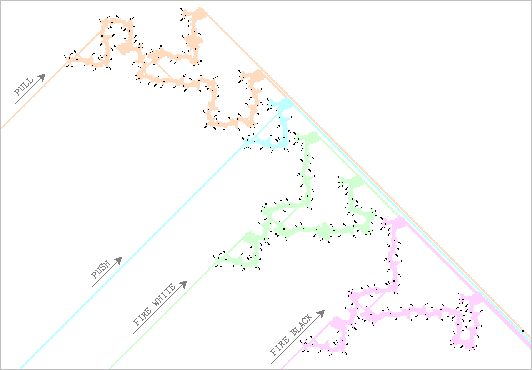
\includegraphics[width=\textwidth]{universal_construction/construction_arm.pdf}}
	\caption{A \textbf{construction arm}, which takes a glider on one or two of four input glider lanes and as a result either pulls or pushes the sliding elbow block (circled in \bgbox{redback}{red}), or uses it to fire a perpendicular glider of either color to the southwest. Note that all four actions require the \texttt{PULL} circuit to be activated, as it produces the frontmost pair of gliders in all four operations (see Exercise~\ref{exer:construction_arm_lanes_timed}). Constructed by Paul Chapman and Dave Greene in 2004.}\label{fig:construction_arm}
\end{figure}

By making use of this construction arm, we can use slow salvo syntheses in which gliders come in from just one or two out of four specified lanes to simulate general slow salvo glider syntheses (in which the gliders can come from any lane). For example, by aiming the output gliders of two construction arms at each other, we can encode any two-direction slow salvo synthesis in the sequence of $4$ input lanes that are used, much like we used armless construction to encode the synthesis of a $2$-engine Cordership in some glider sequences back in Figure~\ref{fig:armless_cordership_gun}.

The pattern displayed in Figure~\ref{fig:mwss_universal_constructor} illustrates how this technique can be used to build a middleweight spaceship gun. While this gun is much larger and more complicated than other MWSS guns that we have seen, it has the advantage that the MWSS is encoded entirely in the input glider streams. To instead have this gun fire a different type of spaceship, or even produce essentially any arrangement of objects in the upper-central quarter of the Life plane, we do not need to change its circuitry at all---only the order in which slow gliders are fed into it (see Exercise~\ref{exer:mwss_universal_constructor_turn_into_other}).

\begin{figure}[!htb]
	\centering
	\embedlink{mwss_universal_constructor}{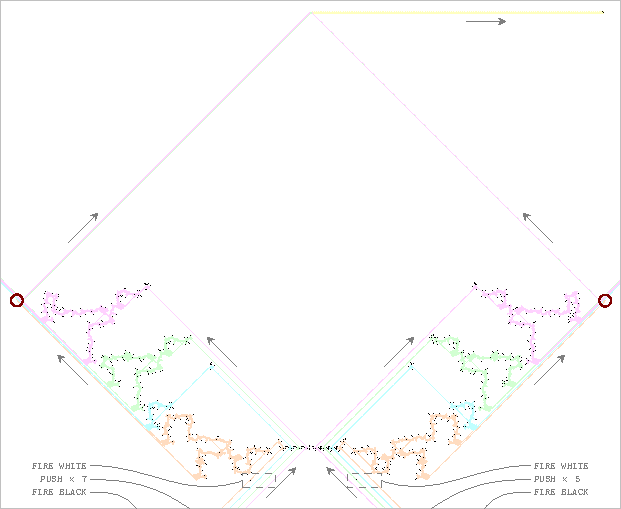
\includegraphics[width=\textwidth]{universal_construction/mwss_universal_constructor.pdf}}
	\caption{A pair of construction arms that are aimed at each other so they can implement two-direction slow salvo syntheses. Here, we first fire a glider from each of the construction arms so as to synthesize a blinker, and then we adjust the positions of the sliding blocks and fire another from each of the construction arms so as to turn that blinker into the middleweight spaceship highlighted in \bgbox{yellowback2}{yellow} (via the incremental synthesis of Table~\ref{tab:sequential_synth}).}\label{fig:mwss_universal_constructor}
\end{figure}


%%%%%%%%%%%%%%%%%%%%%%%%%%%%%%%%
\subsection{The Gemini Itself}\label{sec:gemini_itself}
%%%%%%%%%%%%%%%%%%%%%%%%%%%%%%%%

We can use arrangements of construction arms like the one in Figure~\ref{fig:mwss_universal_constructor} to construct anything that has a glider synthesis. In particular, because these construction arms are made up of such simple components (mostly blocks and eater~1s, with the most difficult piece to synthesize being a tub), they can even be used to synthesize copies of \emph{themselves}. Indeed, this is the key idea behind the Gemini spaceship: use an extremely long chain of gliders to have two construction arms build copies of themselves somewhere else in the plane. To turn this idea into a \emph{spaceship} though (i.e., to make the construction propagate from one location in the Life plane to another, without leaving anything behind itself), we need to make two additions:\smallskip

\begin{itemize}
	\item We need to destroy the original pair of construction arms after they have constructed the new ones. To do this, we simply use a third construction arm (which we will instead call the \textbf{destruction arm}),\index{destruction arm} which is constructed alongside the original pair. After all three arms are constructed, the first two start construction again while the third one starts destroying the no-longer-needed circuitry from the spaceship's previous period. Since objects like blocks and eater~1s can easily be destroyed by a single glider each, it is straightforward to find a glider recipe that destroys these old circuits.\smallskip
	
	\item We need to be able to re-use the glider recipes that store the construction and destruction recipes. Since we cannot use a static loop (we need the glider recipes to move along with the construction arms), we instead have the glider recipes bounce back and forth between \emph{two} copies of the entire three-arm circuit that we have described.\footnote{In fact, the two ends of the spaceship that we construct will be exactly identical. This is the reason for its name ``Gemini''---it is Latin for ``twins''.}\smallskip
\end{itemize}

After we put all of these ideas together, we get the Gemini spaceship that is displayed in Figure~\ref{fig:gemini}.\footnote{Constructed by Andrew J.~Wade in May 2010.} It builds a copy of itself displaced by $5{\thousep}120$ cells in one direction and $1{\thousep}024$ cells in the other direction every $33{\thousep}699{\thousep}586$ generations, making it the first spaceship that we have seen that does not travel orthogonally or diagonally at a slope of~$1$ (its slope is $5120/1024 = 5$).

\begin{figure}[!htb]
	\centering
	\embedlink{gemini}{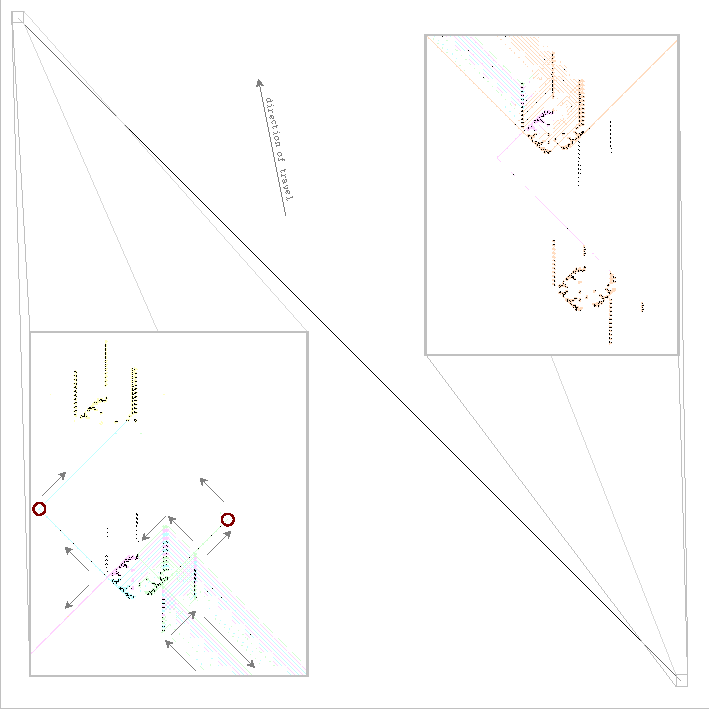
\includegraphics[width=\textwidth]{universal_construction/gemini.pdf}}
	\caption{The self-constructing \textbf{Gemini} spaceship, which simply looks like a long, thin diagonal line when zoomed out far enough to see in its entirety. The bulk of the spaceship of made up of 24 parallel glider lanes (12 travelling in each direction), which carry a recipe for building the ship. The ends of the spaceship, which are zoomed in on here, are identical arrangements of stable glider reflectors, glider duplicators, and three construction/destruction arms whose sliding blocks are circled in \bgbox{redback}{red}. The construction arms highlighted in \bgbox{aquaback}{aqua} and \bgbox{greenpastel}{green} build the next copy of the spaceship (highlighted in \bgbox{yellowback2}{yellow}), while the destruction arm higlighted in \bgbox{magentaback}{magenta} destroys the previous copy of the spaceship (highlighted in \bgbox{orangeback2}{orange}).}\label{fig:gemini}
\end{figure}


%%%%%%%%%%%%%%%%%%%%%%%%%%%%%%%%
\subsection{Geminoids}\label{sec:geminoids}\index{geminoid}
%%%%%%%%%%%%%%%%%%%%%%%%%%%%%%%%

The Gemini spaceship travels at a speed of $(1024,5120)c/33699586$, but it can be modified in numerous ways to produce closely-related spaceships, called \textbf{Geminoids}, that have a wide variety of different speeds and directions. We now explore some of these alterations, and discuss what their theoretical limits are.

The simplest way to change the speed of the Gemini is to change the distance between its two identical ends, without changing any of the glider recipes that bounce back and forth between them. Each additional cell (i.e., full diagonal) by which we separate the ends increases the travel time of each glider by $8$~generations per period ($4$~generations in each direction). Since this change does not affect how far the Gemini travels over the course of its period, this lets us build Geminoids that are arbitrarily slow, having any speed of the form $(1024,5120)c/(33699586 + 8k)$, where $k \geq 0$ is an integer.\footnote{For some values of $k$, we will have to adjust the spacing of the gliders along the track. This is because one of the construction arms at the Gemini's southeast end crosses over the $24$ glider lanes, which can lead to unwanted collisions if we are not careful. Any value of $k$ that is a multiple of $144$ is safe though, as that is the spacing between gliders on those lanes.} We can similarly squeeze the ends of the Gemini closer together, which \emph{decreases} its period by $8$ generation per full diagonal, but only by a bit. The glider sequence still has to fit between the two ends---if we squeeze them too close together then gliders will try to use circuitry before it is constructed (see Exercise~\ref{exer:squeeze_gemini_how_far}).

We can also change the slope (i.e., the direction) that the Gemini travels at, just by changing how many \texttt{PUSH} operations are applied to the northwest construction elbow (i.e., the aqua elbow, in the orientation and coloring scheme of the Gemini displayed in Figure~\ref{fig:gemini}) before it starts constructing. In particular, if it is pushed out $m$ cells before beginning construction, then the resulting displacement of the Geminoid will be $(m-2048,m+2048)$ cells per period.\footnote{When we talk about the northwest elbow being pushed by $m$ cells before constructing, we really just mean that the displacement of the Geminoid over the course of one period is $m$ full diagonals in the northwest direction (i.e., we are working in a coordinate system that is rotated $45$~degrees from the usual one).}

In the Gemini itself, the northwest construction elbow is pushed out by $m = 3072$ cells, for a displacement of $(m-2048,m+2048) = (1024,5120)$ cells per period, and a slope of $5120/1024 = 5$. We can change this into, for example, a knightship\index{knightship} (i.e., a spaceship with slope $2$) by increasing $m$ so that $m+2048 = 2(m-2048)$ (i.e., $m = 6144$). The easiest way to do this is to insert another $3072$ \texttt{PUSH} operations on the northwest construction elbow's path of the Gemini. This alteration produces the knightship Geminoid with $m = 3072 + 3072 = 6144$ and $n = 2048$ (i.e., a displacement of $(4096,8192)$ cells per period) that is displayed in Figure~\ref{fig:geminoid_knightship}.\footnote{This knightship was constructed by Dave Greene in June 2010.}

\begin{figure}[!htb]
	\centering
	\embedlink{geminoid_knightship}{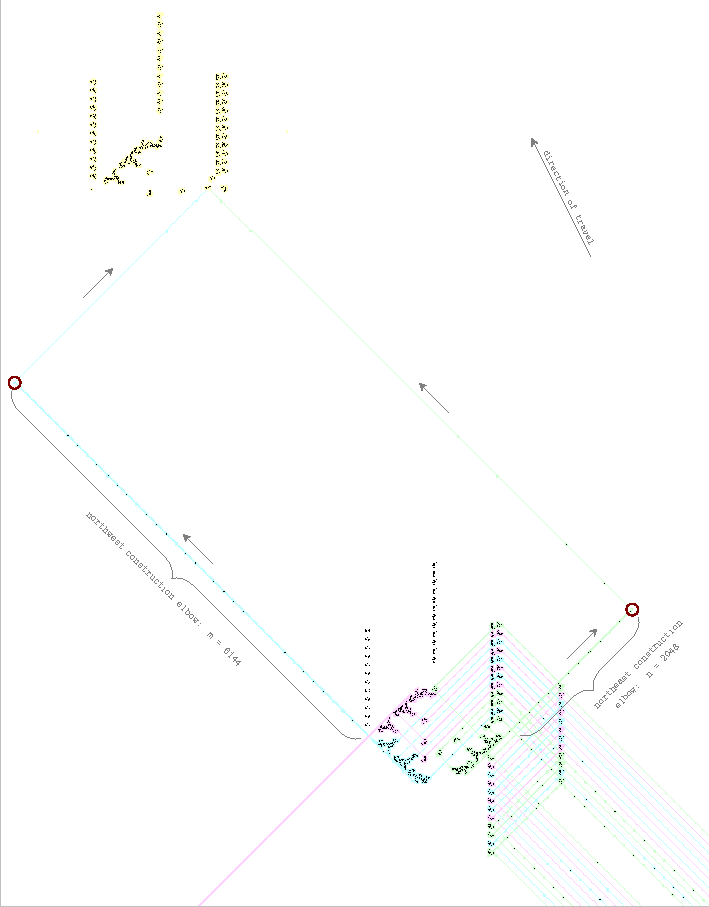
\includegraphics[width=\textwidth]{universal_construction/geminoid_knightship.pdf}}
	\caption{The northwest corner of a (slope $2$) knightship Geminoid. It functions the exact same as the Gemini itself from Figure~\ref{fig:gemini}, except the construction elbow along the \bgbox{aquaback}{aqua} path is pushed an extra $3072$ full diagonals before beginning construction. It travels at a speed of $(4096,8192)c/35567490$.}\label{fig:geminoid_knightship}
\end{figure}

We can achieve an even wider variety of Geminoid slopes by similarly pushing the northeast construction elbow (i.e., the green one in Figures~\ref{fig:gemini} and~\ref{fig:geminoid_knightship}) farther out before construction begins. We have to be slightly more careful with this elbow, though, for two reasons:\smallskip

\begin{itemize}
	\item To keep the two halves of the Geminoid lined up properly, we cannot just push the northeast construction elbow away by $n$ cells---we also have to push the three rows of reflectors and glider duplicators on the northeast half of those ends away by $n/2$ cells.\footnote{And $n$ must therefore be even.}\smallskip
	
	\item The destruction elbow must be pushed out by the same amount as the northeast construction elbow: $n$ cells. Furthermore, the destruction recipe itself must be changed slightly to accommodate the fact that the circuits that it is destroying have been separated by $n/2$ cells (see the above bullet).\smallskip
\end{itemize}

If we (carefully, taking into account the technicalities mentioned above) push out the northwest and northeast construction elbows by $m$ and $n$ cells, respectively, the resulting Geminoid will have a displacement of $(m-n,m+n)$ cells per period. Its slope will thus be $(m+n)/(m-n)$,\footnote{If $m = n$ then the Geminoid will travel straight up, orthogonally.} so any rational slope $p/q \neq 1$ (i.e., diagonal) is attainable: we can get any rational slope $p/q$ that is larger than $1$ by choosing $m = 2p+2q$ and $n = 2p-2q$, so that
\[
	\frac{m+n}{m-n} = \frac{(2p+2q)+(2p-2q)}{(2p+2q)-(2p-2q)} = \frac{4p}{4q} = \frac{p}{q},
\]
and we can achieve any rational slope that is between $0$ and $1$ by rotating one of these Geminoids by $90$~degrees.

In addition to changing Gemini's slope, we can also use this method of inserting additional \texttt{PUSH} operations to increase its speed. For example, if we insert another $3072$ \texttt{PUSH} operations on the Gemini's northwest construction elbow's path, and another $2048$ \texttt{PUSH} operations on its northeast construction elbow's path (i.e., we increase the construction elbow displacements to $m = 6144$ and $n = 4096$), we get a Geminoid that travels exactly twice as far as the Gemini per period: $(2048,10240)$. The exact speed of this new Geminoid depends a bit on some fine details like how much space we leave between the new \texttt{PUSH}-triggering gliders, and how tightly we push the ends of the Geminoid together, but it will be a bit under twice as fast as the original Gemini.

By adding more and more \texttt{PUSH} operations to each of the construction elbows, we can construct Geminoids that travel faster and faster. However, this speed increase is limited by the speed at which we can perform consecutive \texttt{PUSH} operations. Since the Gemini's circuitry contains a Callahan G-to-H\index{Callahan G-to-H} (refer back to Figure~\ref{fig:callahan_g_to_h}), which has a repeat time of $575$ generations, any \texttt{PUSH}-triggering gliders that we add to the Gemini must be separated by at least that much. Furthermore, since each \texttt{PUSH} operation pushes the elbow $1$ full diagonal farther away, it adds an extra $4$ generations to the Gemini's period, for a total of $575+4 = 579$~generations per \texttt{PUSH}. When we put all of these observations together, we arrive at the following theorem:

\begin{theorem}[Geminoid Speed Limit]\label{thm:geminoid_speed_limit}
	By changing the locations at which the Gemini spaceship constructs its circuitry (but without changing the components of that circuitry), we can construct Geminoid spaceships with any speed of the form $(x,y)c$, where $x, y < 1/579$ are rational numbers with $x \neq y$.
\end{theorem}

If we are willing to further tweak our Geminoids then we could make ones that are even faster, though the rebuilding effort would increase considerably. For example, we could replace the Callahan G-to-H that is used in the Gemini's construction arms with a Silver reflector, thus bringing its repeat time down to $497$~generations, and its asymptotic speed limit up to $c/(497+4) = c/501$.

We could even go one step further and replace all reflectors that are used in the Gemini by Snarks, and all glider duplicators by syringe-based conduits (like the upcoming Scorbie splitter in Section~\ref{sec:scorbie_splitter}). The resulting circuitry's repeat time would then be $90$~generations, for an asymptotic speed limit of the Geminoid equal to $c/(90+4) = c/94$. However, a Geminoid with a speed anywhere close to this limit would have to be monstrously large due to the high number of \texttt{PUSH} operations used each period. Furthermore, it would require a complete rebuild of the Gemini, and extreme care would have to be taken to avoid unwanted collisions in the now more-tightly-packed crossing glider streams.\footnote{These crossing glider streams make it rather fiddly to even reduce the spacing between gliders from $576$~generations in the current Gemini to the theoretically possible $575$~generations.}


%%%%%%%%%%%%%%%%%%%%%%%%%%%%%%%%
\section{Single-Channel Glider Synthesis with a 90-Degree Elbow}\label{sec:single_channel_synth}\index{elbow}\index{90-degree elbow}\index{single-channel synthesis}
%%%%%%%%%%%%%%%%%%%%%%%%%%%%%%%%

While Geminoids let us construct spaceships that travel in any direction, they all travel quite slowly. We now switch gears and start developing the tools needed to construct a new type of spaceship that travels at any speed (but not any direction) of our choosing.

Recall from Section~\ref{sec:slow_salvo} that slow salvo synthesis is a method of encoding the construction of a pattern in the positions of a sequence gliders, with their timing playing no role (except that the gap between consecutive gliders must be sufficiently large that each glider's collision must settle down before the next glider arrives). We now flip this idea around and instead show how to encode the construction of a pattern in the \emph{timing} of a sequence of gliders, with their \emph{position} playing no role. In particular, we show how to encode glider synthesis via gliders that are all coming from the same direction on the same lane.


%%%%%%%%%%%%%%%%%%%%%%%%%%%%%%%%
\subsection{Creating Slow 90-Degree Gliders}\label{sec:single_channel_create_perp_glider}
%%%%%%%%%%%%%%%%%%%%%%%%%%%%%%%%

As with many of our other universal constructions, we make use of a block that acts as an elbow in order to make these single-lane syntheses possible. In particular, we fire a stream of gliders at a block so as to first create a chaotic explosion (by turning the block into a pi-heptomino), and then clean up the resulting debris while creating a perpendicular glider. For example, Figure~\ref{fig:90_degree_first_example} displays a sequence of 13~gliders that, when it collides with a block, produces a single glider travelling in a different direction.

\begin{figure}[!htb]
	\centering
	\patternlink{90_degree_first_example}{\vcenteredhbox{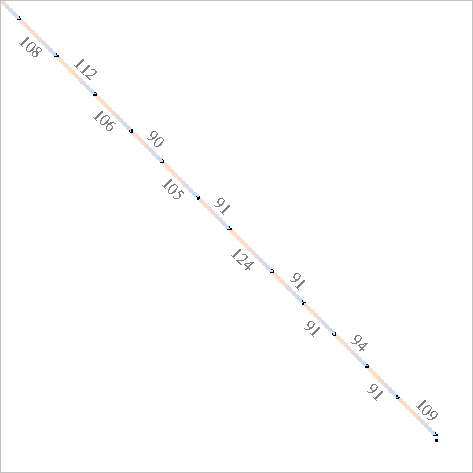
\includegraphics[width=0.486864\textwidth]{universal_construction/90_degree_first_example.pdf}} \vcenteredhbox{\begin{tabular}{@{}c@{}}\color{black}{$\xrightarrow{\text{\clock{3}{3} 1186}}$} \\ \gliderarrow{13}\end{tabular}} \vcenteredhbox{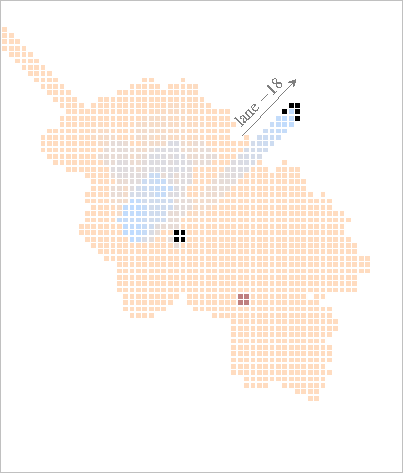
\includegraphics[width=0.414736\textwidth]{universal_construction/90_degree_first_example_2.pdf}}}
	\caption{A sequence of $13$ gliders travelling along the same lane that collide with a block so as to (a) produce a single perpendicular glider, and (b) recreate the target block along the same lane (but shifted northwest by 20 half-diagonals) so that it can be re-used by other single-channel recipes. The numbers on the left indicate the number of generations between consecutive gliders.}\label{fig:90_degree_first_example}
\end{figure}

Since all gliders in a single-channel recipe like this come from the same direction on the same lane, we can encode it simply via the number of generations between each consecutive pair of gliders. For example, the $13$-glider recipe from Figure~\ref{fig:90_degree_first_example} could be encoded by the following sequence of $12$~timing gaps:
\begin{center}
	\texttt{109, 91, 94, 91, 91, 124, 91, 105, 90, 106, 112, 108}.
\end{center}

Computer searches have been carried out\footnote{Mostly by Simon Ekstr{\"o}m, with some optimizations by Dave Greene, in 2017.} to generate single-channel glider recipes that, when aimed at a block as in Figure~\ref{fig:90_degree_first_example} (i.e., so that the first glider triggers a block-to-pi-heptomino explosion), a single output glider is produced on some perpendicular lane. A summary of some reasonably short recipes of this type that produce gliders on a variety of different output lanes (and in either of the two perpendicular output directions) is provided in Table~\ref{tab:single_lane_90deg_glider_timings}.

\newcolumntype{L}{>{\hspace*{-\tabcolsep}}r}
\newcolumntype{R}{l<{\hspace*{-\tabcolsep}}}
\begin{table}[!htb]
	\centering
	\begin{tabular}{@{\hskip 0.31cm}L@{\hskip 0.27cm}r@{\hskip 0.27cm}R@{\hskip 0.34cm}}\toprule
		Lane & Move & Timings \\\midrule
		\texttt{-18i} & \texttt{-20} & \footnotesize\texttt{109,91,94,91,91,124,91,105,90,106,112,108,{\color{gray}(90)}}\\
		\rowcolor{gray!20}\texttt{-15i} & \texttt{-4} & \footnotesize\texttt{109,90,93,91,91,92,90,90,91,90,110,90,90,91,124,133,90,91,113,90,90,{\color{gray}(90)}}\\
		\texttt{-7i} & \texttt{-25} & \footnotesize\texttt{109,91,94,91,91,136,91,90,91,104,90,90,90,110,90,90,98,{\color{gray}(90)}}\\
		\rowcolor{gray!20}\texttt{1i} & \texttt{2} & \footnotesize\texttt{109,91,94,91,90,96,90,91,146,240,109,91,94,91,91,92,90,143,90,91,158,{\color{gray}(90)}}\\
		\texttt{3i} & \texttt{-27} & \footnotesize\texttt{109,90,93,91,91,142,90,109,91,92,90,92,90,118,91,91,90,90,119,{\color{gray}(90)}}\\
		\rowcolor{gray!20}\texttt{5i} & \texttt{8} & \footnotesize\texttt{109,91,94,91,91,136,91,90,91,139,98,90,156,{\color{gray}(133)}}\\
		\texttt{8i} & \texttt{-8} & \footnotesize\texttt{109,90,95,245,90,126,208,128,90,96,91,90,90,91,91,91,91,100,90,90,{\color{gray}(90)}}\\
		\rowcolor{gray!20}\texttt{19i} & \texttt{15} & \footnotesize\texttt{109,91,94,91,91,92,90,97,91,90,91,90,149,90,98,91,90,95,{\color{gray}(90)}}\\\midrule
		\texttt{-21x} & \texttt{-37} & \footnotesize\texttt{109,91,93,90,155,106,90,90,92,91,109,90,93,91,90,100,124,{\color{gray}(90)}}\\
		\rowcolor{gray!20}\texttt{-15x} & \texttt{-26} & \footnotesize\texttt{109,91,93,91,127,91,90,113,90,90,111,90,111,91,91,91,{\color{gray}(90)}}\\
		\texttt{-11x} & \texttt{8} & \footnotesize\texttt{109,91,94,91,91,136,91,90,91,101,90,90,90,92,90,144,90,91,90,90,126,{\color{gray}(90)}}\\
		\rowcolor{gray!20}\texttt{-9x} & \texttt{16} & \footnotesize\texttt{109,91,94,91,91,136,91,90,91,168,90,90,97,91,91,91,90,116,90,90,90,90,90,{\color{gray}(90)}}\\
		\texttt{-3x} & \texttt{-15} & \footnotesize\texttt{109,91,93,91,97,91,91,106,91,90,90,90,90,90,91,163,90,90,104,{\color{gray}(90)}}\\
		\rowcolor{gray!20}\texttt{-1x} & \texttt{-5} & \footnotesize\texttt{109,91,94,91,91,136,91,90,91,139,98,90,94,90,95,90,91,118,207,93,{\color{gray}(90)}}\\
		\texttt{2x} & \texttt{3} & \footnotesize\texttt{109,91,94,91,91,92,90,143,90,91,158,{\color{gray}(90)}}\\
		\rowcolor{gray!20}\texttt{10x} & \texttt{11} & \footnotesize\texttt{109,91,94,91,91,92,90,119,90,90,109,91,94,91,91,92,90,143,90,91,158,{\color{gray}(90)}}\\
		\bottomrule
	\end{tabular}
	\caption{Single-channel glider recipes that collide with a 90-degree elbow so as to produce a perpendicular output glider on a given lane. The first 8 rows give recipes that produce an ``\textbf{i}nternal'' glider (i.e., one that travels northeast when oriented as in Figure~\ref{fig:90_degree_first_example}) and the last 8 rows give sequences that produce an ``e\textbf{x}ternal'' glider (i.e., one that travels southwest). The ``move'' column indicates how many half-diagonals the elbow is moved forward, and the ``timings'' column indicates the number of generations between consecutive gliders in the sequence. The final number in parentheses is the number of generations that must pass before it is safe to send subsequent glider recipes.}\label{tab:single_lane_90deg_glider_timings}
\end{table}

There are numerous points of clarification that we need to make about these recipes:\smallskip

\begin{itemize}
	\item The output lane number has either an ``\texttt{i}'' or ``\texttt{x}'' suffix, indicating in which of the two perpendicular directions the output glider travels. The suffixes stand for \textbf{i}nternal and e\textbf{x}ternal, which refer to the output glider travelling on the same side as the elbow block that the input glider sequence hits, or the opposite side, respectively.\smallskip 
	
	\item Some of these glider sequences, like the one with output on lane~2x, change the zero-degree elbow block into another small object like a boat, beehive, or pond. This is okay because those objects explode into a pi-heptomino when they are hit by a glider in the exact same way that a block does, and this is always the reaction that the first glider in these single-channel sequence triggers.\smallskip
	
	\item The ``move'' column of Table~\ref{tab:single_lane_90deg_glider_timings} specifies how many half-diagonals farther away the zero-degree elbow is moved by the glider sequence. If this value is odd then the elbow is moved to the other side of the input glider stream. If this happens, the output lanes of all subsequent glider sequences are flipped from \texttt{i} to \texttt{x}, and vice-versa. For example, the sequence corresponding to lane~$2x$ has a ``move'' value of $3$, which is odd. Thus if we want to output gliders on lanes $2x$ and then $-12x$, we would have to send the sequences corresponding to lanes $2x$ and then $-15i$ (not $-15x$).\smallskip
	
	\item In most of these glider sequences, there are numerous gaps of 90 and 91~generations. The reason for this is that we want to be able to feed these single-channel glider recipes through standard components like Snarks and the easy-to-synthesize Lx200-assisted\index{Lx200} syringe\index{syringe} from Exercise~\ref{exer:syringe_Lx200} (which has a repeat time of~$90$ generations).\footnote{Single-channel glider sequences with large timing gaps are desirable since they can make use of circuitry that has a higher repeat time. We could use sequences with gaps no smaller than $153$~generations (such sequences are known to be able to emulate arbitrary glider syntheses), thus letting us feed these sequences through the syringe variant from Figure~\ref{fig:syringe_modified}, for example. However, as the minimum timing gap increases, so does the length of the resulting glider sequences, so we stick with a minimum timing gap of 90~generations.} Most of the gliders that have a timing of 90 or 91 generations could actually be moved much closer (i.e., the previous glider's collision settles down before they arrive), but only if they are used on conjunction with faster-recovering conduits. The reason that some gliders use a gap of $91$~generations instead of just $90$ is that their timing matters mod~$2$, due to p$2$ components like blinkers in an intermediate reaction.\smallskip
\end{itemize}


%%%%%%%%%%%%%%%%%%%%%%%%%%%%%%%%
\subsection{Moving the Elbow}\label{sec:single_channel_move_elbow}
%%%%%%%%%%%%%%%%%%%%%%%%%%%%%%%%

The sequences given in Table~\ref{tab:single_lane_90deg_glider_timings} can only be used to fire gliders on a small selection of lanes (8 in each direction). Furthermore, these sequences move the elbow forward and backward by some amount that we do not control---it is dictated by the output lane on which we wish to fire a glider. It is thus important to be able to move the elbow however far forward or backward we like, \emph{without} firing a glider, so that the glider-firing sequences then produce a glider where we actually want it. For example, the following pair of elbow-moving sequences, which are displayed in Figure~\ref{fig:0_degree_block_push_pull}, move the elbow forward by $8$~half diagonals or backward by $12$ half diagonals, respectively.
\begin{align*}
& \text{\texttt{~push~8hd: \footnotesize 109, 91, 94, 91, 91, 92, 90, 119, 90, {\color{gray}(90)},}}\\
& \text{\texttt{pull~12hd: \footnotesize 109, 91, 93, 91, 137, 91, 91, 125, 172, 108, 90, 109, 91, 101, 120, 90, {\color{gray}(90)}.}}
\end{align*}

\begin{figure}[!htb]
	\centering
	\begin{tabular}{@{}cc@{}}
		\begin{subfigure}{0.48\textwidth}
			\centering
			\patternlink{0_degree_block_push}{\vcenteredhbox{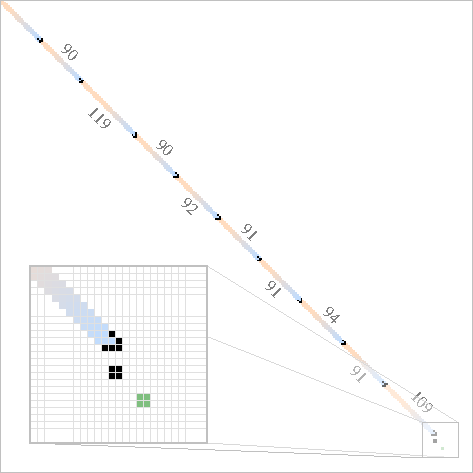
\includegraphics[width=\textwidth]{universal_construction/0_degree_block_push.pdf}}}
			\caption{push 8 half diagonals}
			\label{fig:0_degree_block_push}
		\end{subfigure} & \begin{subfigure}{0.48\textwidth}
			\centering
			\patternlink{0_degree_block_pull}{\vcenteredhbox{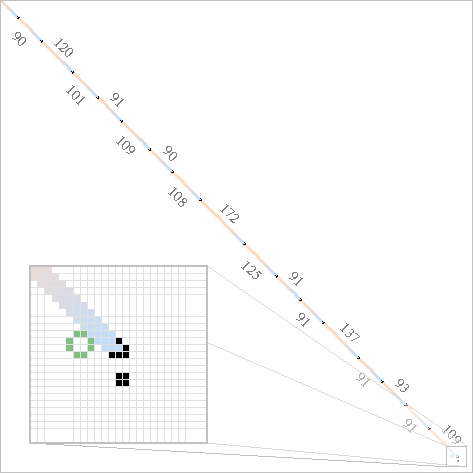
\includegraphics[width=\textwidth]{universal_construction/0_degree_block_pull.pdf}}}
			\caption{pull 12 half diagonals}
			\label{fig:0_degree_block_pull}
		\end{subfigure}
	\end{tabular}
	\caption{Single-channel glider sequences that (a) push or (b) pull an elbow. The location of the elbow after being pushed or pulled is marked in \bgbox{greenpastel}{green}.}\label{fig:0_degree_block_push_pull}
\end{figure}

A more complete summary of elbow-moving sequences is given in Table~\ref{tab:single_lane_elbow_movers}, which tells us how to move the $90$-degree elbow in either direction by any number of half-diagonals up to $10$. To move the elbow by a larger amount, we can simply repeat these sequences.

\begin{table}[!htb]
	\centering
	\begin{tabular}{@{\hskip 0.31cm}L@{\hskip 0.27cm}R@{\hskip 0.34cm}}\toprule
		Move & Timings \\\midrule
		\texttt{-10} & \footnotesize\texttt{109,91,94,91,91,96,90,97,91,91,130,94,90,105,90,95,111,{\color{gray}(90)}}\\
		\rowcolor{gray!20} \texttt{-9} & \footnotesize\texttt{109,91,94,91,91,179,90,91,94,91,102,91,105,91,108,90,91,91,120,90,{\color{gray}(90)}}\\
		\texttt{-8} & \footnotesize\texttt{109,90,93,91,90,95,91,90,91,91,90,90,91,90,90,99,90,90,91,90,94,90,{\color{gray}(90)}}\\
		\rowcolor{gray!20} \texttt{-7} & \footnotesize\texttt{109,91,93,91,118,90,91,91,91,90,90,156,114,90,90,90,90,141,{\color{gray}(90)}}\\
		\texttt{-6} & \footnotesize\texttt{109,91,93,91,156,91,91,94,90,91,140,91,103,91,91,132,{\color{gray}(90)}}\\
		\rowcolor{gray!20} \texttt{-5} & \footnotesize\texttt{109,91,94,91,91,92,90,173,100,90,141,91,90,90,90,147,90,117,{\color{gray}(192)}}\\
		\texttt{-4} & \footnotesize\texttt{109,90,93,91,91,90,90,92,90,95,91,170,90,90,91,91,98,91,91,{\color{gray}(90)}}\\
		\rowcolor{gray!20} \texttt{-3} & \footnotesize\texttt{109,91,94,91,90,96,90,91,92,90,217,90,103,{\color{gray}(90)}}\\
		\texttt{-2} & \footnotesize\texttt{109,91,94,91,91,136,90,90,91,171,100,118,90,{\color{gray}(90)}}\\
		\rowcolor{gray!20} \texttt{-1} & \footnotesize\texttt{109,91,94,91,90,96,90,91,146,{\color{gray}(240)}}\\\midrule
		\texttt{1} & \footnotesize\texttt{109,91,94,91,91,92,90,143,90,91,156,90,104,{\color{gray}(164)}}\\
		\rowcolor{gray!20} \texttt{2} & \footnotesize\texttt{109,90,93,91,91,90,90,91,91,90,90,91,90,90,94,90,{\color{gray}(90)}}\\
		\texttt{3} & \footnotesize\texttt{109,91,94,91,91,92,90,143,90,90,90,129,101,102,{\color{gray}(90)}}\\
		\rowcolor{gray!20} \texttt{4} & \footnotesize\texttt{109,91,93,91,92,90,90,90,151,93,90,143,134,94,90,90,90,109,91,{\color{gray}(90)}}\\
		\texttt{5} & \footnotesize\texttt{109,91,93,91,92,90,110,90,152,90,90,91,91,91,90,90,90,90,175,119,115,{\color{gray}(193)}}\\
		\rowcolor{gray!20} \texttt{6} & \footnotesize\texttt{109,91,93,91,145,215,104,90,90,90,90,90,102,92,90,90,90,106,155,150,{\color{gray}(90)}}\\
		\texttt{7} & \footnotesize\texttt{109,91,94,91,90,96,90,91,146,240,109,91,94,91,91,92,90,119,90,{\color{gray}(90)}}\\
		\rowcolor{gray!20} \texttt{8} & \footnotesize\texttt{109,91,94,91,91,92,90,119,90,{\color{gray}(90)}}\\
		\texttt{9} & \footnotesize\texttt{109,90,93,91,91,90,90,95,90,91,90,90,140,90,90,128,{\color{gray}(93)}}\\
		\rowcolor{gray!20} \texttt{10} & \footnotesize\texttt{109,91,93,91,129,149,91,90,90,105,90,90,90,90,114,91,100,90,{\color{gray}(90)}}\\\bottomrule
	\end{tabular}
	\caption{Single-channel glider sequences that can be used to move the 90-degree elbow to any location along the input glider lane. The ``move'' and ``timings'' columns are as in Table~\ref{tab:single_lane_90deg_glider_timings}.}\label{tab:single_lane_elbow_movers}
\end{table}

With these block-moving sequences at our disposal, we are now able to use gliders on a single lane to fire slow perpendicular gliders on any sequence of lanes of our choosing: by repeating the sequences from Table~\ref{tab:single_lane_elbow_movers} we can move the elbow to any lane that we like, and we can then use a sequence from Table~\ref{tab:single_lane_90deg_glider_timings} to  actually fire a perpendicular glider.


%%%%%%%%%%%%%%%%%%%%%%%%%%%%%%%%
\subsection{Creating and Using a Hand}\label{sec:single_channel_hand}
%%%%%%%%%%%%%%%%%%%%%%%%%%%%%%%%

The only extra ingredient that we need in order to show that single-channel glider synthesis with a 90-degree elbow block is universal (i.e., can implement any glider synthesis) is a way of creating a target block (which we refer to as a \textbf{hand}\footnote{It is connected to an elbow, after all.})\index{hand} that the perpendicular slow gliders will be fired at. One sequence of gliders that works to create such a hand block is
\begin{align}\begin{split}\label{eq:make_hand_90_deg}
& \text{\texttt{109, 91, 93, 90, 132, 115, 127, 91, 90, 91, 95, 90, 114,}} \\
& \text{\texttt{~~~~~~~~~162, 233, 159, 90, 155, 126, 93, 118, 90, 91, 90, {\color{gray}(90)},}}
\end{split}\end{align}
which is illustrated as the first transition in Figure~\ref{fig:90_degree_block_move}. Indeed, this recipe creates a hand block $86$ half-diagonals away, on the internal side of the elbow block, while pushing that elbow block away by $17$ half~diagonals.\footnote{In particular, since we have described the elbow block as moving by an odd number of half-diagonals, we know that it moves to the opposite side of the single-lane glider sequence.}

Since we can now use single-channel glider sequences and a $90$-degree elbow to create slow gliders on any lane, and we can also create a hand block for those gliders to collide with, we immediately see from Theorem~\ref{thm:p1_slow_salvo} that these types of glider syntheses are universal. That is, we have demonstrated the following result:

\begin{theorem}[Universality of Single-Channel Synthesis]\label{thm:single_channel_90_degree}
	Every pattern that can be constructed via glider synthesis can be constructed by a single-channel glider synthesis with a $90$-degree elbow.
\end{theorem}

To illustrate how to implement slow salvo synthesis via single-channel synthesis, consider the problem of moving the hand block after we create it. We can use any of the slow salvos from Figures~\ref{fig:block_movers} and~\ref{fig:p2_block_movers} to carry out this task---we will implement the $4$-glider $(11,0)$ block pull\index{(11,0) block pull} from Figure~\ref{fig:block_move_11_0}, which uses gliders on lanes (relative to the initial position of the elbow block) $-6i$, $-6i$, $6i$, and $0i$, in that order.

To this end, we first use the hand-making sequence of gliders~\eqref{eq:make_hand_90_deg}, which moves the block to position~$17$. We then fire the four slow gliders as follows:\smallskip

\begin{itemize}
	\item We want to fire a glider $17 - (-6) = 23$ lanes behind the elbow. Since the hand-making sequence of gliders flipped the orientation of the elbow block, we thus want to fire the first glider on lane $-23x$ (not $-23i$). This can be achieved by a $-2$ half-diagonal elbow move (from Table~\ref{tab:single_lane_elbow_movers}) followed by firing a glider on lane $-21x$ (from Table~\ref{tab:single_lane_90deg_glider_timings}).\smallskip
	
	\item Since firing a glider on lane $-21x$ moved the elbow by $-37$ half-diagonals (which is odd, so the elbow's orientation is flipped back to where it started), the elbow is now on lane $17 - 2 - 37 = -22$. We want to fire a glider $-22 - (-6) = -16$ lanes behind the elbow, which is lane $16i$. This can be achieved by pushing the elbow forward by $8$hd and then firing on lane $8i$.\smallskip
	
	\item Since firing on lane $8i$ moved the elbow by $-8$hd, it is now on lane $-22 + 8 - 8 = -22$. We want to fire a glider $-22 - 6 = -28$ lanes behind the elbow, which is lane $28i$. This can be achieved by pushing the elbow forward by $10$hd, pushing it by $10$hd again, and then firing on lane $8i$.\footnote{Be careful---we cannot just push the elbow forward by $9$hd and then fire on lane $19i$, since the $9$hd move would flip the orientation of the block, meaning you would have to fire on lane $19x$ instead.}\smallskip
	
	\item Finally, since firing on lane $8i$ moved the elbow backward by $8$hd, it is now on lane $-22 + 10 + 10 - 8 = -10$. We want to fire a glider $-10 - 0 = -10$ lanes behind the elbow, which is lane $10i$. This can be achieved by a $2$hd elbow move followed by firing a glider on lane $8i$.\smallskip
\end{itemize}

When we put all of this together, we get the following single-lane sequence of 185 gliders (which we illustrate in Figure~\ref{fig:90_degree_block_move} and specify by 184 timings between those gliders) that first creates a hand block and then moves that hand block $11$~cells via a sequence of $4$ perpendicular slow gliders:\footnote{We did something slightly tricky with with the two ``move 10hd'' sequences here---notice that the gap between their final pair of gliders are not the same as each other. See Exercise~\ref{exer:single_lane_glider_final_glider_explain}.}
\begin{align*}
& \text{\texttt{\footnotesize make hand: {\scriptsize 109, 91, 93, 90, 132, 115, 127, 91, 90, 91, 95, 90, 114, 162, 233, 159, 90, 155, 126, 93,}}} \\
& \text{\texttt{\footnotesize ~~~~~~~~~~~~{\scriptsize 118, 90, 91, 90, 90,}}} \\
& \text{\texttt{\footnotesize move -2hd: {\scriptsize 109, 91, 94, 91, 91, 136, 90, 90, 91, 171, 100, 118, 90, 90,}}} \\
& \text{\texttt{\footnotesize fire -21x: {\scriptsize 109, 91, 93, 90, 155, 106, 90, 90, 92, 91, 109, 90, 93, 91, 90, 100, 124, 90,}}} \\
& \text{\texttt{\footnotesize move~~8hd: {\scriptsize 109, 91, 94, 91, 91, 92, 90, 119, 90, 90,}}} \\
& \text{\texttt{\footnotesize fire~~~8i: {\scriptsize 109, 90, 95, 245, 90, 126, 208, 128, 90, 96, 91, 90, 90, 91, 91, 91, 91, 100, 90, 90, 90,}}} \\
& \text{\texttt{\footnotesize move~10hd: {\scriptsize 109, 91, 93, 91, 129, 149, 91, 90, 90, 105, 90, 90, 90, 90, 114, 91, 100, 90, 90,}}} \\
& \text{\texttt{\footnotesize move~10hd: {\scriptsize 109, 91, 93, 91, 129, 149, 91, 90, 90, 105, 90, 90, 90, 90, 114, 91, 100, 90, 91,}}} \\
& \text{\texttt{\footnotesize fire~~~8i: {\scriptsize 109, 90, 95, 245, 90, 126, 208, 128, 90, 96, 91, 90, 90, 91, 91, 91, 91, 100, 90, 90, 90,}}} \\
& \text{\texttt{\footnotesize move~~2hd: {\scriptsize 109, 90, 93, 91, 91, 90, 90, 91, 91, 90, 90, 91, 90, 90, 94, 90, 90,}}} \\
& \text{\texttt{\footnotesize fire~~~8i: {\scriptsize 109, 90, 95, 245, 90, 126, 208, 128, 90, 96, 91, 90, 90, 91, 91, 91, 91, 100, 90, 90.}}}
\end{align*}

\begin{figure}[!htb]
	\centering
	\embedlink{90_degree_block_move}{\vcenteredhbox{\phantom{$\cdots$ $\xrightarrow{\text{\clock{2}{12} 1720}}$}} \vcenteredhbox{\patternimg{0.07}{90_degree_block_move_0}} \vcenteredhbox{\begin{tabular}{@{}c@{}}\color{black}{$\xrightarrow{\text{\clock{7}{1} 2859}}$} \\ \gliderarrow{25}\end{tabular}} \vcenteredhbox{\patternimg{0.07}{90_degree_block_move_1}} \vcenteredhbox{\begin{tabular}{@{}c@{}}\color{black}{$\xrightarrow{\text{\clock{11}{20} 1448}}$} \\ \gliderarrow{14}\end{tabular}} \vcenteredhbox{\patternimg{0.07}{90_degree_block_move_2}}} \\[1em]
	
	\patternlink{90_degree_block_move}{\vcenteredhbox{\begin{tabular}{@{}c@{}}\color{black}{$\cdots$ $\xrightarrow{\text{\clock{2}{12} 1720}}$} \\ \hphantom{$\cdots$} \gliderarrow{18}\end{tabular}} \vcenteredhbox{\patternimg{0.07}{90_degree_block_move_3}} \vcenteredhbox{\begin{tabular}{@{\hskip 0.09cm}c@{\hskip 0.09cm}}\color{black}{$\xrightarrow{\text{\clock{1}{52} 973}}$} \\ \gliderarrow{10}\end{tabular}} \vcenteredhbox{\patternimg{0.07}{90_degree_block_move_4}} \vcenteredhbox{\begin{tabular}{@{}c@{}}\color{black}{$\xrightarrow{\text{\clock{9}{25} 2266}}$} \\ \gliderarrow{21}\end{tabular}} \vcenteredhbox{\patternimg{0.07}{90_degree_block_move_5}}} \\[1em]
	
	\patternlink{90_degree_block_move}{\vcenteredhbox{\begin{tabular}{@{}c@{}}\color{black}{$\cdots$ $\xrightarrow{\text{\clock{2}{12} 1903}}$} \\ \hphantom{$\cdots$} \gliderarrow{19}\end{tabular}} \vcenteredhbox{\patternimg{0.07}{90_degree_block_move_6}} \vcenteredhbox{\begin{tabular}{@{}c@{}}\color{black}{$\xrightarrow{\text{\clock{2}{13} 1904}}$} \\ \gliderarrow{19}\end{tabular}} \vcenteredhbox{\patternimg{0.07}{90_degree_block_move_7}} \vcenteredhbox{\begin{tabular}{@{}c@{}}\color{black}{$\xrightarrow{\text{\clock{9}{25} 2266}}$} \\ \gliderarrow{21}\end{tabular}} \vcenteredhbox{\patternimg{0.07}{90_degree_block_move_8}}} \\[1em]
	
	\patternlink{90_degree_block_move}{\vcenteredhbox{\begin{tabular}{@{}c@{}}\color{black}{$\cdots$ $\xrightarrow{\text{\clock{8}{5} 1565}}$} \\ \hphantom{$\cdots$} \gliderarrow{17}\end{tabular}} \vcenteredhbox{\patternimg{0.07}{90_degree_block_move_9}} \vcenteredhbox{\begin{tabular}{@{}c@{}}\color{black}{$\xrightarrow{\text{\clock{9}{25} 2266}}$} \\ \gliderarrow{21}\end{tabular}} \vcenteredhbox{\patternimg{0.07}{90_degree_block_move_10}} \vcenteredhbox{\color{black}{\hspace{0.08cm}$\xrightarrow{\text{\clock{6}{45} 138}}$\hspace{0.08cm}}} \vcenteredhbox{\patternimg{0.07}{90_degree_block_move_11}}}
	
	\caption{A single-lane sequence of 185 gliders creating a hand block and then firing 4 perpendicular slow gliders at that hand block so as to move it down by 11~cells. The perpendicular slow gliders are created on the correct lanes by repeatedly adjusting the position of the 90-degree elbow.}\label{fig:90_degree_block_move}
\end{figure}



%%%%%%%%%%%%%%%%%%%%%%%%%%%%%%%%
\section{Single-Channel Glider Synthesis with a Zero-Degree Elbow}\label{sec:single_channel_synth_0}\index{zero-degree elbow}
%%%%%%%%%%%%%%%%%%%%%%%%%%%%%%%%

While the single-channel syntheses of the previous subsection are very useful, it is sometimes desirable to use single-channel glider recipes to build an object directly in front of them, rather than off to their side. For example, it will be useful for us to be able to use gliders from a single lane to construct a Snark that accepts gliders on that same lane as input. To make this possible, instead of using a 90-degree elbow we use a \textbf{zero-degree elbow}:\index{zero-degree elbow} a small stable object (like a block) that several gliders are fired at on a particular lane so as to produce a single glider going in the \emph{same direction} but on a different lane.\footnote{Here, ``zero-degree'' refers to the fact that the input glider stream is being ``reflected'' by zero degrees (i.e., not reflected at all, but just shifted to a different lane).}


%%%%%%%%%%%%%%%%%%%%%%%%%%%%%%%%
\subsection{Creating Slow Zero-Degree Gliders}\label{sec:single_channel_zero_make_slow}
%%%%%%%%%%%%%%%%%%%%%%%%%%%%%%%%

To illustrate how a zero-degree elbow works, consider the sequence of $14$~gliders displayed in Figure~\ref{fig:lane_8_0degree} that, when it collides with a block, produces a single glider going in the same direction, but shifted by $8$ lanes.

\begin{figure}[!htb]
	\centering
	\patternlink{lane_8_0degree}{\vcenteredhbox{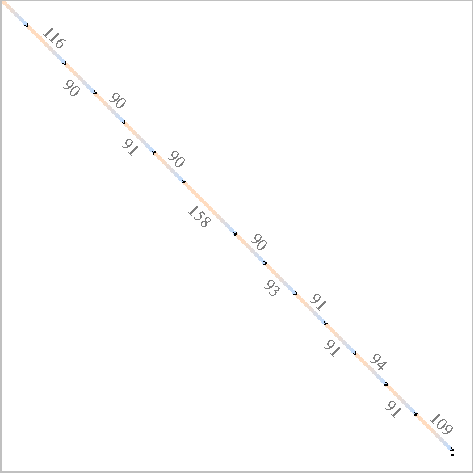
\includegraphics[width=0.4508\textwidth]{universal_construction/lane_8_0degree.pdf}}  \vcenteredhbox{\begin{tabular}{@{}c@{}}\color{black}{$\xrightarrow{\text{\clock{3}{3} 1440}}$} \\ \gliderarrow{14}\end{tabular}} \vcenteredhbox{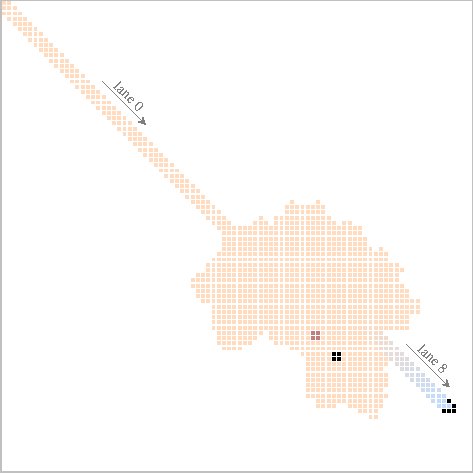
\includegraphics[width=0.4508\textwidth]{universal_construction/lane_8_0degree_2.pdf}}}
	\caption{A sequence of $14$ gliders travelling along the same lane that collide with a block so as to (a) produce a single glider travelling in the same direction, but shifted up by $8$~lanes, and (b) recreate the target block along the same lane (but shifted southeast by 8 half-diagonals) so that it can be re-used by other single-channel recipes.}\label{fig:lane_8_0degree}
\end{figure}

As with $90$-degree single-channel sequences, we encode zero-degree single-channel sequences simply by the number of generations between each consecutive pair of gliders. For example, we encode the $14$-glider sequence from Figure~\ref{fig:lane_8_0degree} via the following sequence of $13$~timing gaps:
\begin{center}
	\texttt{109, 91, 94, 91, 91, 93, 90, 158, 90, 91, 90, 90, 116, {\color{gray}(104)}},
\end{center}
with the final number in gray indicating how many generations must pass before another glider sequence can safely arrive.

In this zero-degree setting, it is much more important to be able to fire output gliders on a wide variety of different lanes than it was in the 90-degree setting. Indeed, when we worked with a 90-degree elbow we were able to simply move the elbow forward or backward to reach different output lanes, but doing so has no effect whatsoever on the output lane in the zero-degree setting.

For this reason, extensive computer searches have been used to generate single-channel glider sequences of this type that produce a single output glider on any lane from $-100$ to $+100$.\footnote{A complete collection of tens of thousands of these recipes can be downloaded from \httpsurl{gitlab.com/apgoucher/slmake/-/tree/master/data/simeks}. It can be useful to have multiple recipes for the same output lane, since they might move the zero-degree elbow by different amounts.} A summary of sequences of this type for output lanes $-22$ through $+22$ is provided in Table~\ref{tab:single_lane_0deg_glider_timings}.

\begin{table}[!phtb]
	\centering
	\begin{tabular}{@{\hskip 0.31cm}L@{\hskip 0.27cm}r@{\hskip 0.27cm}R@{\hskip 0.34cm}}\toprule
		Lane & Move & Timings \\\midrule
		\texttt{-22} & \texttt{-20} & \footnotesize\texttt{109,91,94,91,91,136,90,90,91,114,90,91,90,99,90,97,90,90,90,126,90,137,90,{\color{gray}(90)}} \\
		\rowcolor{gray!20}\texttt{-21} & \texttt{8} & \footnotesize\texttt{109,91,94,91,91,95,91,90,146,91,99,90,118,120,135,90,90,121,{\color{gray}(90)}} \\
		\texttt{-20} & \texttt{-29} & \footnotesize\texttt{93,90,91,91,90,90,91,90,103,113,91,103,90,152,181,140,91,90,166,91,{\color{gray}(106)}} \\
		\rowcolor{gray!20}\texttt{-19} & \texttt{-20} & \footnotesize\texttt{109,91,93,91,171,91,90,90,94,91,106,91,91,90,90,143,90,91,91,91,90,91,112,{\color{gray}(90)}} \\
		\texttt{-18} & \texttt{8} & \footnotesize\texttt{109,90,93,91,91,128,91,91,90,97,90,99,90,139,91,91,117,134,92,90,90,90,{\color{gray}(90)}} \\
		\rowcolor{gray!20}\texttt{-17} & \texttt{-22} & \footnotesize\texttt{109,91,93,91,123,90,129,90,90,111,142,91,90,120,91,142,{\color{gray}(98)}} \\
		\texttt{-16} & \texttt{8} & \footnotesize\texttt{109,91,94,91,91,124,91,126,91,140,162,148,90,90,119,90,{\color{gray}(90)}} \\
		\rowcolor{gray!20}\texttt{-15} & \texttt{13} & \footnotesize\texttt{109,91,93,90,156,91,91,94,91,90,147,117,91,144,90,91,128,100,91,90,105,91,{\color{gray}(90)}} \\
		\texttt{-14} & \texttt{-39} & \footnotesize\texttt{109,91,93,91,155,106,91,91,96,90,90,91,108,90,156,90,90,120,90,112,91,99,{\color{gray}(90)}} \\
		\rowcolor{gray!20}\texttt{-13} & \texttt{1} & \footnotesize\texttt{109,91,93,91,92,90,158,90,94,270,172,130,90,91,91,96,90,90,147,{\color{gray}(90)}} \\
		\texttt{-12} & \texttt{-23} & \footnotesize\texttt{109,91,94,91,90,162,122,111,90,90,90,96,91,91,91,122,91,91,171,{\color{gray}(90)}} \\
		\rowcolor{gray!20}\texttt{-11} & \texttt{-53} & \footnotesize\texttt{93,91,151,90,139,180,103,115,167,91,120,139,135,91,91,{\color{gray}(169)}} \\
		\texttt{-10} & \texttt{15} & \footnotesize\texttt{109,91,93,91,97,91,90,91,120,90,95,91,143,90,90,90,90,{\color{gray}(90)}} \\
		\rowcolor{gray!20}\texttt{-9} & \texttt{-15} & \footnotesize\texttt{109,91,94,91,91,90,91,91,90,158,90,91,90,90,101,90,107,90,90,90,{\color{gray}(90)}} \\
		\texttt{-8} & \texttt{1} & \footnotesize\texttt{93,91,116,90,106,91,143,91,109,90,91,103,110,91,136,91,92,91,155,{\color{gray}(199)}} \\
		\rowcolor{gray!20}\texttt{-7} & \texttt{-34} & \footnotesize\texttt{109,91,93,91,92,91,98,201,91,129,90,90,90,90,90,103,90,108,90,104,{\color{gray}(90)}} \\
		\texttt{-6} & \texttt{-11} & \footnotesize\texttt{109,91,94,91,90,90,90,90,109,91,101,90,98,90,{\color{gray}(90)}} \\
		\rowcolor{gray!20}\texttt{-5} & \texttt{-20} & \footnotesize\texttt{109,91,94,91,91,95,91,90,104,90,90,97,91,91,94,191,97,90,126,{\color{gray}(90)}} \\
		\texttt{-4} & \texttt{-23} & \footnotesize\texttt{0,93,91,90,144,90,111,91,92,91,103,91,144,90,168,91,91,102,90,92,90,94,{\color{gray}(90)}} \\
		\rowcolor{gray!20}\texttt{-3} & \texttt{-9} & \footnotesize\texttt{109,91,94,91,91,136,90,90,91,168,90,106,90,90,138,90,90,106,{\color{gray}(90)}} \\
		\texttt{-2} & \texttt{7} & \footnotesize\texttt{109,91,93,91,92,91,90,90,162,91,91,90,129,91,113,90,90,90,{\color{gray}(90)}} \\
		\rowcolor{gray!20}\texttt{-1} & \texttt{-9} & \footnotesize\texttt{109,90,95,245,90,95,90,123,91,90,115,142,{\color{gray}(90)}} \\\midrule
		\texttt{0} & \texttt{-1} & \scriptsize\texttt{109,91,93,91,92,90,97,91,116,91,145,90,91,98,90,90,188,91,90,90,{\color{gray}(90)}} \\\midrule
		\rowcolor{gray!20}\texttt{1} & \texttt{-24} & \scriptsize\texttt{109,91,94,91,91,93,90,95,90,113,90,99,90,156,90,90,90,138,{\color{gray}(170)}} \\
		\texttt{2} & \texttt{-27} & \scriptsize\texttt{109,91,94,91,91,124,91,90,91,91,90,91,90,141,90,172,91,161,90,169,228,{\color{gray}(90)}} \\
		\rowcolor{gray!20}\texttt{3} & \texttt{4} & \scriptsize\texttt{109,91,94,91,91,92,90,169,90,90,90,107,90,90,91,90,95,91,{\color{gray}(90)}} \\
		\texttt{4} & \texttt{-56} & \scriptsize\texttt{109,91,94,91,91,92,90,169,91,90,116,90,161,91,104,{\color{gray}(90)}} \\
		\rowcolor{gray!20}\texttt{5} & \texttt{-8} & \footnotesize\texttt{109,90,93,91,91,135,91,124,90,90,148,91,91,97,141,91,{\color{gray}(90)}} \\
		\texttt{6} & \texttt{-15} & \scriptsize\texttt{93,90,90,90,91,90,91,136,155,98,120,90,90,91,92,90,97,161,161,{\color{gray}(139)}} \\
		\rowcolor{gray!20}\texttt{7} & \texttt{-30} & \footnotesize\texttt{109,91,94,91,91,124,91,105,90,169,91,90,116,91,142,90,90,{\color{gray}(90)}} \\
		\texttt{8} & \texttt{8} & \scriptsize\texttt{109,91,94,91,91,93,90,158,90,91,90,90,116,{\color{gray}(104)}} \\
		\rowcolor{gray!20}\texttt{9} & \texttt{11} & \footnotesize\texttt{109,91,93,90,171,90,90,91,90,91,90,91,129,144,90,90,120,90,91,91,169,90,{\color{gray}(90)}} \\
		\texttt{10} & \texttt{14} & \scriptsize\texttt{109,91,93,90,140,150,108,91,90,111,91,91,194,98,90,169,{\color{gray}(90)}} \\
		\rowcolor{gray!20}\texttt{11} & \texttt{-5} & \scriptsize\texttt{109,91,94,91,91,92,90,146,90,90,90,91,135,91,152,{\color{gray}(135)}} \\
		\texttt{12} & \texttt{8} & \scriptsize\texttt{91,94,91,91,121,90,90,90,90,90,90,99,90,165,119,90,106,90,90,{\color{gray}(90)}} \\
		\rowcolor{gray!20}\texttt{13} & \texttt{-32} & \scriptsize\texttt{109,91,94,91,91,96,90,97,91,91,145,90,113,90,90,105,91,193,{\color{gray}(90)}} \\
		\texttt{14} & \texttt{-16} & \scriptsize\texttt{109,91,93,91,129,149,91,90,90,142,219,90,99,91,109,115,92,185,{\color{gray}(90)}} \\
		\rowcolor{gray!20}\texttt{15} & \texttt{9} & \scriptsize\texttt{109,90,93,91,91,158,94,113,91,90,91,96,90,142,{\color{gray}(90)}} \\
		\texttt{16} & \texttt{8} & \scriptsize\texttt{109,91,94,91,91,95,91,90,93,218,172,90,90,90,116,112,341,107,106,90,163,91,{\color{gray}(90)}} \\
		\rowcolor{gray!20}\texttt{17} & \texttt{-28} & \scriptsize\texttt{109,91,94,91,91,96,90,166,91,91,114,90,90,91,90,90,114,91,101,{\color{gray}(90)}} \\
		\texttt{18} & \texttt{1} & \scriptsize\texttt{109,90,93,91,91,148,91,90,151,90,91,163,108,151,112,144,90,149,90,90,99,{\color{gray}(90)}} \\
		\rowcolor{gray!20}\texttt{19} & \texttt{-19} & \scriptsize\texttt{109,91,93,91,115,107,90,90,90,90,90,90,90,103,99,118,91,130,{\color{gray}(90)}} \\
		\texttt{20} & \texttt{12} & \scriptsize\texttt{109,91,93,90,169,90,91,103,91,133,90,90,91,91,90,110,91,93,90,112,171,{\color{gray}(90)}} \\
		\rowcolor{gray!20}\texttt{21} & \texttt{-2} & \scriptsize\texttt{109,91,93,91,120,91,91,91,91,90,91,100,91,90,97,91,91,90,90,{\color{gray}(160)}} \\
		\texttt{22} & \texttt{27} & \scriptsize\texttt{109,91,94,91,91,93,90,91,91,90,100,90,94,90,108,90,91,91,119,{\color{gray}(90)}} \\\bottomrule
	\end{tabular}
	\caption{Single-channel glider sequences that produce an output glider on a given lane (relative of the sequence itself, which is on lane~0). The ``move'' and ``timings'' columns are as in Table~\ref{tab:single_lane_90deg_glider_timings}.}\label{tab:single_lane_0deg_glider_timings}
\end{table}

As with 90-degree single-lane sequences, the value in the ``move'' column being odd means that the zero-degree elbow moves to the other side of the input glider stream. If this happens, the output lanes of all subsequent glider sequences are flipped from positive to negative, and vice-versa. For example, the sequence corresponding to lane~2 has a ``move'' value of $-27$, which is odd. If we want to output gliders on lanes $2$ and then $3$, we would thus have to send the sequences corresponding to lanes $2$ and then $-3$ (not $3$).\footnote{Since the ``move'' value for the lane~$-3$ sequence is also odd, the zero-degree elbow would then be back on its original side of the glider stream after this second sequence.}


%%%%%%%%%%%%%%%%%%%%%%%%%%%%%%%%
\subsection{Moving the Elbow}\label{sec:single_channel_zero_move_elbow}
%%%%%%%%%%%%%%%%%%%%%%%%%%%%%%%%

Unlike a $90$-degree elbow, we typically do not care about the exact position of the zero-degree elbow.\footnote{This is one feature that makes zero-degree elbows easier to work with than $90$-degree elbows.} Indeed, rather than having to align the elbow with a particular output lane, we just have to make sure that the elbow stays within an acceptable region---we do not want to move it so far forward that it crashes into whatever we are constructing, nor so far backward that it crashes into the source of the gliders. Fortunately, the elbow-moving sequences that we already saw in Table~\ref{tab:single_lane_elbow_movers} (or even just the two sequences from Figure~\ref{fig:0_degree_block_push_pull}) can be used to adjust the positioning of the elbow if needed.


%%%%%%%%%%%%%%%%%%%%%%%%%%%%%%%%
\subsection{Creating and Using a Hand}\label{sec:single_channel_zero_make_hand}
%%%%%%%%%%%%%%%%%%%%%%%%%%%%%%%%

Now that we can create output gliders on a wide variety of different lanes, we need to be able to create a target for those output gliders to hit. Once again, this target (typically a block) is called a \textbf{hand},\index{hand} but this time we must build it in front of the elbow rather than off to its side.\footnote{Technically, we \emph{could} use the same hand block~\eqref{eq:make_hand_90_deg} that we used with the $90$-degree elbow, since that hand is within the $-100$ to $+100$ lane range that we can fire output gliders on via the zero-degree elbow. However, it is much more convenient to use a more centered hand instead.} One sequence that creates a suitable hand block is provided below and illustrated in Figure~\ref{fig:0degree_hand}:
\begin{center}
	\texttt{\small 109, 90, 93, 91, 91, 90, 90, 100, 90, 90, 146, 96, 90, 90, 90, 92, 156, 144, {\color{gray}(90)}}.
\end{center}

\begin{figure}[!htb]
	\centering
	\patternlink{0degree_hand}{\vcenteredhbox{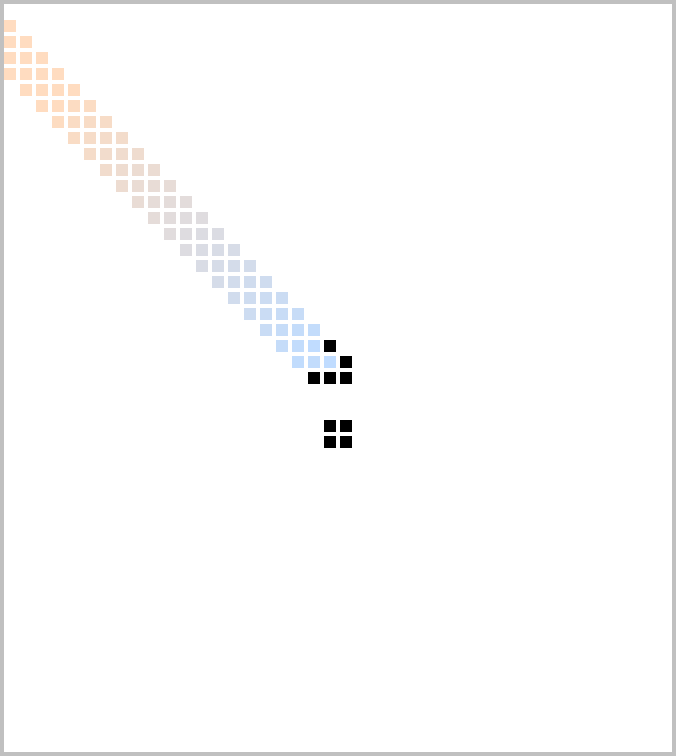
\includegraphics[width=0.3\textwidth]{universal_construction/0degree_hand.png}} \vcenteredhbox{\begin{tabular}{@{}c@{}}\color{black}{$\xrightarrow{\text{\clock{3}{35} 1868}}$} \\ \gliderarrow{19}\end{tabular}} \vcenteredhbox{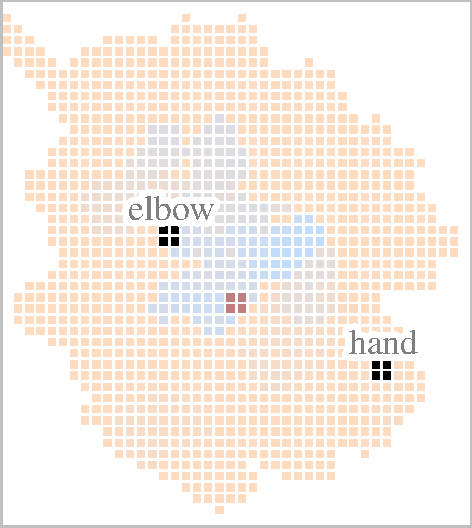
\includegraphics[width=0.3\textwidth]{universal_construction/0degree_hand_2.pdf}}}
	\caption{A single-lane sequence of $19$ gliders creating a hand block for a zero-degree elbow.}\label{fig:0degree_hand}
\end{figure}

Since the hand that this glider sequence creates is fairly close to the zero-degree elbow, it is often a good idea to separate them a bit more by applying one of the elbow-pulling sequences that we have seen. We can use the $12$hd pull from Figure~\ref{fig:0_degree_block_pull}, for example, repeatedly to create as large of a gap between the elbow and hand as we want.

With the glider sequences that we have now seen, it is straightforward to use a zero-degree elbow to synthesize any object that has a slow salvo synthesis no wider than $200$ or so lanes.\footnote{It is actually possible to use a zero-degree elbow to implement \emph{any} slow salvo synthesis (i.e., zero-degree elbows are universal, just like we saw $90$-degree elbows are universal in Theorem~\ref{thm:single_channel_90_degree}). Indeed, we could use the zero-degree elbow to fire a slow salvo that duplicates the hand block, thus leaving us with \emph{three} blocks: the zero-degree elbow block, which fires at a (slow, not single-lane) $90$-degree elbow block, which fires at a target block. However, actually synthesizing anything in this manner is excruciatingly slow, so we do not make use of this technique.} For example, we implement the $4$-glider $(11,0)$ block pull\index{(11,0) block pull} from Figure~\ref{fig:block_move_11_0} via a zero-degree elbow much like we did for the $90$-degree elbow. However, the details work out more simply since we do not have to worry about moving the elbow to a precise location after each slow glider is produced:\smallskip

\begin{itemize}
	\item We first use the hand-making sequence of gliders from Figure~\ref{fig:0degree_hand}. We then want to fire gliders on lanes~$-1$, $-1$, $11$, and $5$, in that order.\smallskip
	
	\item To fire a glider on lane~$-1$, we simply use the appropriate glider sequence from Table~\ref{tab:single_lane_0deg_glider_timings}.\smallskip
	
	\item To fire another glider on lane~$-1$, we have to instead use the glider sequence corresponding to lane~$1$ (since the zero-degree elbow was moved to the other side of the glider sequence in the previous step, which has an odd ``move'' value of $-9$). However, before we can fire this glider, we have to pull the elbow block away from the hand block, or else they would collide with each other at this point. We thus apply the $12$hd pull sequence from Figure~\ref{fig:0_degree_block_pull} twice.\smallskip
	
	\item To fire the third glider on lane $11$, we use the glider sequence corresponding to lane $-11$ (since the elbow block is still on the side of the glider sequence opposite from where it started).\smallskip
	
	\item Since the lane~$-11$ sequence pulled the elbow block by $53$ half-diagonals (which is odd), the zero-degree elbow has now been flipped back to its original side of the glider sequence. We can thus simply use the glider sequence corresponding to lane~$5$ at this point.\smallskip
\end{itemize}

When we put all of this together, we get the following single-lane sequence of $118$ gliders (which we illustrate in Figure~\ref{fig:0_degree_block_move} and specify by $117$ timings between those gliders) that first creates a hand block and then moves that hand block $11$~cells via a sequence of $4$ parallel slow gliders:
\begin{align*}
& \text{\texttt{\footnotesize make hand: {\footnotesize 109, 90, 93, 91, 91, 90, 90, 100, 90, 90, 146, 96, 90, 90, 90, 92, 156, 144, 90,}}} \\
& \text{\texttt{\footnotesize ~fire~~-1: {\footnotesize 109, 90, 95, 245, 90, 95, 90, 123, 91, 90, 115, 142, 90,}}} \\
& \text{\texttt{\footnotesize ~move~-12: {\footnotesize 109, 91, 93, 91, 137, 91, 91, 125, 172, 108, 90, 109, 91, 101, 120, 90, 90,}}} \\
& \text{\texttt{\footnotesize ~move~-12: {\footnotesize 109, 91, 93, 91, 137, 91, 91, 125, 172, 108, 90, 109, 91, 101, 120, 90, 90,}}} \\
& \text{\texttt{\footnotesize ~fire~~~1: {\footnotesize 109, 91, 94, 91, 91, 93, 90, 95, 90, 113, 90, 99, 90, 156, 90, 90, 90, 138, 170,}}} \\
& \text{\texttt{\footnotesize ~fire~-11: {\footnotesize 93, 91, 151, 90, 139, 180, 103, 115, 167, 91, 120, 139, 135, 91, 91, 169,}}} \\
& \text{\texttt{\footnotesize ~fire~~~5: {\footnotesize 109, 90, 93, 91, 91, 135, 91, 124, 90, 90, 148, 91, 91, 97, 141, 91.}}}
\end{align*}

\begin{figure}[!htb]
	\centering
	\embedlink{0_degree_block_move}{\vcenteredhbox{\phantom{$\cdots$ $\xrightarrow{\text{\clock{2}{12} 1904}}$}} \vcenteredhbox{\patternimg{0.069}{0_degree_block_move_0}} \vcenteredhbox{\begin{tabular}{@{}c@{}}\color{black}{$\xrightarrow{\text{\clock{7}{1} 1904}}$} \\ \gliderarrow{19}\end{tabular}} \vcenteredhbox{\patternimg{0.069}{0_degree_block_move_1}} \vcenteredhbox{\begin{tabular}{@{}c@{}}\color{black}{$\xrightarrow{\text{\clock{11}{20} 1447}}$} \\ \gliderarrow{13}\end{tabular}} \vcenteredhbox{\patternimg{0.069}{0_degree_block_move_2}}} \\[1em]
	
	\patternlink{90_degree_block_move}{\vcenteredhbox{\begin{tabular}{@{}c@{}}\color{black}{$\cdots$ $\xrightarrow{\text{\clock{2}{12} 1775}}$} \\ \hphantom{$\cdots$} \gliderarrow{17}\end{tabular}} \vcenteredhbox{\patternimg{0.069}{0_degree_block_move_3}} \vcenteredhbox{\begin{tabular}{@{}c@{}}\color{black}{$\xrightarrow{\text{\clock{2}{12} 1775}}$} \\ \gliderarrow{17}\end{tabular}} \vcenteredhbox{\patternimg{0.069}{0_degree_block_move_4}} \vcenteredhbox{\begin{tabular}{@{}c@{}}\color{black}{$\xrightarrow{\text{\clock{9}{25} 1923}}$} \\ \gliderarrow{19}\end{tabular}} \vcenteredhbox{\patternimg{0.069}{0_degree_block_move_5}}} \\[1em]
	
	\patternlink{90_degree_block_move}{\vcenteredhbox{\begin{tabular}{@{}c@{}}\color{black}{$\cdots$ $\xrightarrow{\text{\clock{8}{5} 1858}}$} \\ \hphantom{$\cdots$} \gliderarrow{16}\end{tabular}} \vcenteredhbox{\patternimg{0.069}{0_degree_block_move_6}} \vcenteredhbox{\begin{tabular}{@{}c@{}}\color{black}{$\xrightarrow{\text{\clock{9}{25} 1664}}$} \\ \gliderarrow{17}\end{tabular}} \vcenteredhbox{\patternimg{0.069}{0_degree_block_move_8}} \vcenteredhbox{\phantom{\color{black}{\hspace{0.08cm}$\xrightarrow{\text{\clock{6}{45} 138}}$\hspace{0.08cm}}}} \vcenteredhbox{\phantom{\patternimg{0.069}{0_degree_block_move_8}}}}
	
	\caption{A single-lane sequence of 118 gliders creating a hand block and then firing 4 parallel slow gliders at that hand block so as to move it up by 11~cells. The parallel slow gliders are created on the correct lanes by using the sequences from Table~\ref{tab:single_lane_0deg_glider_timings}.}\label{fig:0_degree_block_move}
\end{figure}


%%%%%%%%%%%%%%%%%%%%%%%%%%%%%%%%
\section{Duplicating and Reflecting Single-Channel Recipes}\label{sec:snarkmaker}
%%%%%%%%%%%%%%%%%%%%%%%%%%%%%%%%

Now that we know how to build things with single-channel glider recipes, we would like to be able to manipulate them. In particular, it is going to be important that we are able to reflect these recipes and also duplicate them, so that we can use one copy of the recipe to build something while potentially saving the other copy for later use.

Thanks to the fact that these recipes are single-channel, a single Snark can be used to reflect the entire recipe. However, if there is not already a Snark at the location we would like the reflection to take place, we have to be a bit more clever. In this situation, we can use a single-channel recipe to build a Snark directly in the path of the recipe itself, then let an arbitrary number of gliders be reflected by the Snark, and then use another single-channel recipe to destroy the Snark once it is done being useful. The recipes that create and destroy this in-lane Snark are appropriately called the \textbf{Snarkmaker} and \textbf{Snarkbreaker}.


%%%%%%%%%%%%%%%%%%%%%%%%%%%%%%%%
\subsection{The Snarkmaker}\label{sec:snarkmaker_itself}\index{Snarkmaker}
%%%%%%%%%%%%%%%%%%%%%%%%%%%%%%%%

The Snarkmaker can be constructed by first searching for a unidirectional slow-salvo recipe for a Snark, and then using the zero-degree elbow toolkit from the previous section to turn it into a single-lane recipe (at the expense of having many more gliders). One unidirectional slow salvo synthesis of a Snark that works is the $95$-glider monstrosity displayed in Figure~\ref{fig:snark_slow_salvo}.\footnote{This salvo was found by Adam P.~Goucher in March 2017.}

\begin{figure}[!htb]
	\centering
	\embedlink{snark_slow_salvo}{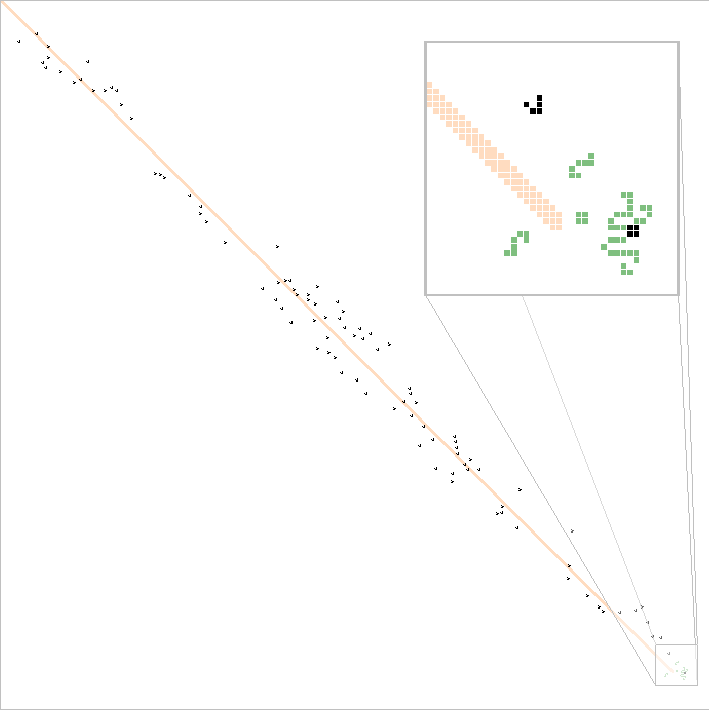
\includegraphics[width=\textwidth]{universal_construction/snark_slow_salvo.pdf}}
	\caption{A $95$-glider unidirectional p$2$ slow salvo synthesis of a Snark. The location of the to-be-constructed Snark is highlighted in \bgbox{greenpastel}{green}, and the lane that it can reflect gliders from is highlighted in \bgbox{orangeback2}{orange}.}\label{fig:snark_slow_salvo}
\end{figure}

We can turn this unidirectional slow salvo into a single-channel recipe by consulting a database of zero-degree single-channel glider sequences. For example, the first glider in the Snark-creating slow salvo is on lane~$15$ (relative to the input lane of the Snark), so it can be created by the lane~$15$ recipe from Table~\ref{tab:single_lane_0deg_glider_timings}:
\begin{center}
	\texttt{\small 109, 90, 93, 91, 91, 158, 94, 113, 91, 90, 91, 96, 90, 142, {\color{gray}(90)}}.
\end{center}
The next glider is on lane~22, so we can again simply use the corresponding recipe from Table~\ref{tab:single_lane_0deg_glider_timings}:
\begin{center}
	\texttt{\small 109, 91, 94, 91, 91, 93, 90, 91, 91, 90, \\ 100, 90, 94, 90, 108, 90, 91, 91, 119, {\color{gray}(90)}}.
\end{center}

After stringing together 95 recipes of this type (one for each glider in the slow salvo),\footnote{This process is completely mechanical, but also extremely tedious, which means it is best done by a computer instead of a human. Also, the particular recipes that we used in the Snarkmaker do not always match up exactly with the recipes from Table~\ref{tab:single_lane_0deg_glider_timings}---multiple recipes are known for most lane numbers.} we get a single-channel recipe consisting of $2{\thousep}253$ gliders that creates a Snark. However, there are still a few other zero-degree elbow recipes that we must prepend and append to make this Snarkmaker actually usable:\smallskip

\begin{itemize}
	\item We first need to use a recipe that creates a block that is offset far to the side, so that the glider recipes that are reflected through the Snark have something to hit (i.e., we need to create a block that will become the 0-degree elbow after the Snark has been made). The 90-degree hand recipe~\eqref{eq:make_hand_90_deg} can carry out this task.\smallskip
	
	\item We then need to use a recipe that creates the zero-degree hand that will be used as the seed for the synthesis of the Snark (i.e., the seed block in Figure~\ref{fig:snark_slow_salvo}). The recipe from Section~\ref{sec:single_channel_zero_make_hand} can carry out this task.\smallskip
	
	\item We need a recipe that can destroy the original zero-degree elbow, since it serves no purpose after the Snark is constructed (and in fact just prevents gliders from entering the Snark). The following 8-glider recipe takes care of this task:
	
	\begin{center}
		\texttt{\small 109, 91, 95, 113, 90, 134, 90, {\color{gray}(90)}}.
	\end{center}
	
	\item Finally, we can use the elbow-moving recipes of Table~\ref{fig:90_degree_block_move} to adjust the relative positioning of the three different elbows that are used throughout all of these operations.\smallskip
\end{itemize}

After we put all of this together, we get a single-channel glider recipe containing a grand total of $2{\thousep}427$ gliders that creates a Snark, and also moves the elbow to its far side so that subsequent glider recipes on that lane hit the elbow after passing through the Snark. This \textbf{Snarkmaker} is displayed in Figure~\ref{fig:snarkmaker}, and the complete sequence of glider timings that make it up is provided in Appendix~\ref{sec:appendix_snarkmaker}.

\begin{figure}[!htb]
	\centering
	\embedlink{snarkmaker}{\vcenteredhbox{\patternimg{0.08}{snarkmaker_0}} \vcenteredhbox{\gliderarrow{56}} \vcenteredhbox{\patternimg{0.08}{snarkmaker_56}} \vcenteredhbox{\gliderarrow{34}} \vcenteredhbox{\patternimg{0.08}{snarkmaker_90}} \\[1em] \vcenteredhbox{\phantom{\patternimg{0.075}{snarkmaker_0}}} \vcenteredhbox{\gliderarrow{2253}} \vcenteredhbox{\patternimg{0.08}{snarkmaker_2343}} \,\! \vcenteredhbox{\gliderarrow{8}} \,\! \vcenteredhbox{\patternimg{0.08}{snarkmaker_2351}}}
	
	\caption{The Snarkmaker, which is a single-channel glider recipe that first creates the post-Snark elbow block, then creates a zero-degree elbow, then creates a Snark via that zero-degree elbow, and then finally destroys the zero-degree elbow. Not displayed are 76 (optional) final gliders that are typically appended at the end to push the post-Snark elbow far enough away from the Snark that another Snarkmaker recipe could be used.}\label{fig:snarkmaker}
\end{figure}

Single-channel recipes are also known for creating a Snark in its three other possible orientations.\footnote{These recipes were all found by Adam P.~Goucher in March 2017---see \httpsurl{conwaylife.com/forums/viewtopic.php?f=2\&t=2660\&start=25\#p42121}.} However, they are all roughly as large as the Snarkmaker, and the details of their construction are all very similar to that of the Snarkmaker, so we do not present them here.



%%%%%%%%%%%%%%%%%%%%%%%%%%%%%%%%
\subsection{The Snarkbreaker}\label{sec:snarkbreaker}\index{Snarkbreaker}
%%%%%%%%%%%%%%%%%%%%%%%%%%%%%%%%

The Snarkbreaker, which destroys a Snark that is in the path a single-channel glider stream, is \emph{considerably} simpler than the Snarkmaker.\footnote{In Life, just like in life, it is typically much easier to break something than it is to make it.} To create it, basically all we need is a way of colliding a glider (or gliders) with the Snark so as to destroy it, and a single-channel recipe that creates those gliders. Recipes that accomplish these tasks, as well as their net effect of converting a Snark back into an elbow block, are displayed in Figure~\ref{fig:snarkbreaker}.

\begin{figure}[!htb]
	\centering
	\embedlink{snarkbreaker}{\phantom{\vcenteredhbox{\gliderarrow{1}}} \vcenteredhbox{\patternimg{0.1}{snarkbreaker_0}} \vcenteredhbox{\gliderarrow{17}} \vcenteredhbox{\patternimg{0.1}{snarkbreaker_17}} \\[1em] \vcenteredhbox{\gliderarrow{1}} \vcenteredhbox{\patternimg{0.1}{snarkbreaker_18}} \,\! \vcenteredhbox{\gliderarrow{2}} \,\! \vcenteredhbox{\patternimg{0.1}{snarkbreaker_20}}}
	
	\caption{The \textbf{Snarkbreaker} is a $20$-glider single-channel recipe that destroys a Snark and turns it back into an elbow block.}\label{fig:snarkbreaker}
\end{figure}

Altogether, the Snarkbreaker consists of 20 gliders, with the following timing gaps:
\begin{align*}
& \text{\texttt{\footnotesize return glider: {\footnotesize 93, 91, 118, 93, 151, 90, 99, 155, 120, 92, 108, 90, 102, 164, 90, 90,}}} \\
& \text{\texttt{\footnotesize Snark destroy: {\footnotesize varies, 143, 97, {\color{gray}(90)}.}}}
\end{align*}
The exact timing of the glider that is labelled ``varies'' depends on how far away the elbow block is from the Snark that is is being used to destroy---the ``varies'' glider must collide with the Snark at the same time as the glider that is fired backward from the elbow by the previous 17 gliders. It follows that if the elbow block is $n$ cells away from the Snark, then the ``varies'' glider must come roughly $8n$ generations after the previous one.



%%%%%%%%%%%%%%%%%%%%%%%%%%%%%%%%
\subsection{The Scorbie Splitter}\label{sec:scorbie_splitter}\index{Scorbie splitter}
%%%%%%%%%%%%%%%%%%%%%%%%%%%%%%%%

The final piece of machinery that we will need for our upcoming constructions is a method of making a single-channel recipe duplicate itself. We have seen numerous methods of duplicating glider streams (e.g., the periodic duplicator of Figure~\ref{fig:periodic_glider_duplicator}, and the stable duplicators of Figure~\ref{fig:glider_multipliers}), but we cannot assume that such mechanisms are already in the path of the single-channel recipe. Instead, we would like to use a single-channel recipe to build a duplicating mechanism in such a way that further recipes along the same lane can make use of it.

The simplest such mechanism to synthesize is called a \textbf{Scorbie splitter},\footnote{Named after Dongook Lee, who uses the ConwayLife.com forums username ``Scorbie''. They were partially responsible for the identification of this conduit and its prominent usage in self-constructing circuitry.} which is displayed in Figure~\ref{fig:scorbie_splitter}. This conduit uses the left half of the large easier-to-synthesize version of the syringe from Figure~\ref{fig:syringe_modified} to convert the input glider into a Herschel, and then another conduit to convert that Herschel into two output gliders (this is the exact same method that was used to create the syringe variant in Exercise~\ref{exer:syringe_Lx200}, and it has the exact same repeat time of $90$~generations as that pattern).

\begin{figure}[!htb]
	\centering
	\patternimglink{0.12}{scorbie_splitter}
	\caption{The \textbf{Scorbie splitter} is a stable glider duplicator that is made up of the left half of a syringe, followed by an H-to-2G conduit on the right that was found by Aidan F.~Pierce in January 2016.}
	\label{fig:scorbie_splitter}
\end{figure}

Just like we can use a single-channel recipe to synthesize a Snark directly on its path, so too can we use such a recipe to synthesize a Scorbie splitter directly on its path. In principle, we could build a recipe to carry out this task by hand---we just need to make a slow salvo synthesis that builds each of the Scorbie splitter's still lifes, one at a time, and then convert that slow-salvo synthesis into a zero-degree single-channel recipe in the same way that we did with the Snarkmaker. However, the computer script \emph{slsparse}\index{slsparse} (see \httpsurl{conwaylife.com/wiki/Slsparse} for tutorials and a download link) automates this procedure and is able to generate single-channel recipes for objects of this size and complexity in a minute or two. One such Scorbie-splitter-making recipe consists of $4{\thousep}006$ gliders, whose timing gaps are provided in Appendix~\ref{sec:appendix_scorbie_splitter_maker}.

We can also use single-channel recipes to synthesize Scorbie splitters in any other orientation, or via a 90-degree elbow instead of a zero-degree elbow. In all cases, the method of construction is basically the same, and slsparse can deal with them straightforwardly---see Exercise~\ref{exer:scorbie_splitter_zero_degree}. In fact, once we figure out how to synthesize an object from one orientation via a single-channel recipe, the other orientations come for free since we can just prepend as many Snarkmakers to the recipe as we need---see Exercise~\ref{exer:why_scorbie_splitter_snarkmakers}.


%%%%%%%%%%%%%%%%%%%%%%%%%%%%%%%%
\section{A Slow Demonoid}\label{sec:slow_demonoid}
%%%%%%%%%%%%%%%%%%%%%%%%%%%%%%%%

The downside of single-channel glider synthesis versus slow salvo synthesis is that the former requires somewhere around $25$ to $40$ times as many gliders to synthesize the same object (roughly the length of an average elbow-moving sequence followed by a glider-firing sequence). However, the upside of it is that the surrounding circuitry that makes use of the synthesis can be considerably simpler, since it just needs to be able to manipulate gliders along a single lane.

We now demonstrate the utility of single-channel glider synthesis by creating another self-constructing spaceship. This spaceship, which is called a \textbf{Demonoid}\footnote{The name \textbf{Demonoid} is a portmanteau of ``diagonal'' and ``Geminoid''.},\index{Demonoid} is smaller than the Gemini by roughly one order of magnitude---it has approximately $7 \times 10^4$ live cells instead of $8 \times 10^5$, and its bounding box has a side length of approximately $3 \times 10^5$ cells instead of $4 \times 10^6$.

Much like the Gemini works by bouncing 12 glider streams back and forth between two identical ends that they construct and destroy, this Demonoid works by bouncing a single-channel recipe back and forth between two mirror-image ends that they construct and destroy. This time, the ends consist just of a Scorbie splitter (to duplicate the single-channel recipe, so that one copy can be used for construction purposes while the other copy is preserved) and a Snark (to send the preserved copy of the single-channel recipe back toward the other end of the Demonoid), as illustrated in Figure~\ref{fig:slow_demonoid}.

\begin{figure}[!htbp]
	\centering
	\embedlink{slow_demonoid}{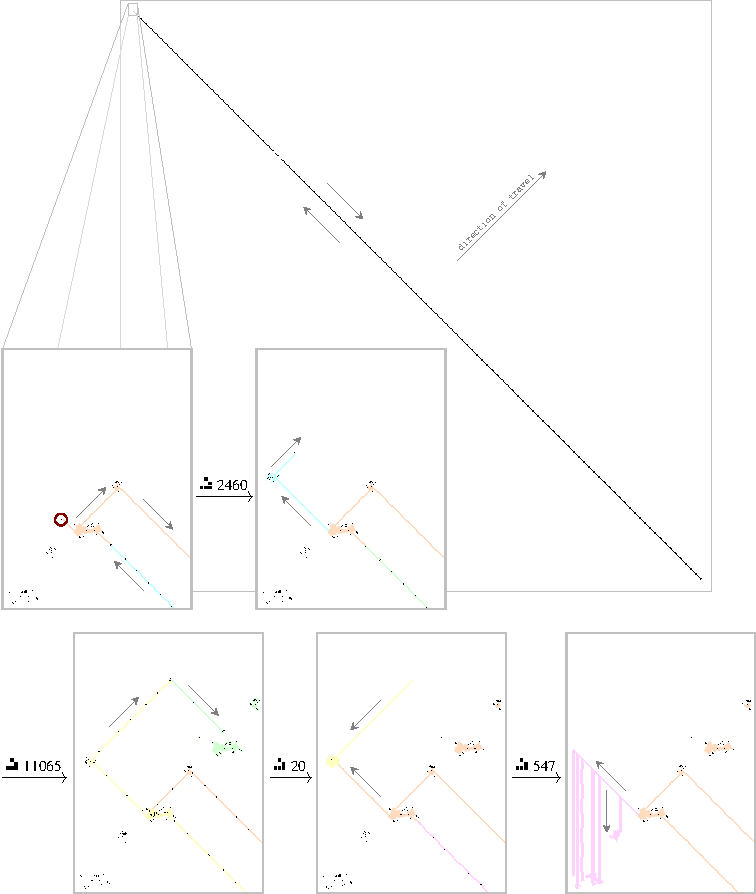
\includegraphics[width=\textwidth]{universal_construction/slow_demonoid.pdf}}
	\caption{A $c/16384$ Demonoid spaceship that works by bouncing a (very long) single-channel glider recipe between two self-constructing ends that are made up of a Scorbie splitter and a Snark. The first $2{\thousep}460$ gliders collide with an elbow block (circled in \bgbox{redback}{red}) so as to build a temporary Snark (highlighted in \bgbox{aquaback}{aqua}) to provide a better angle for construction. The next $11{\thousep}220$ gliders use a $90$-degree elbow to construct the next Scorbie splitter and Snark (highlighted in \bgbox{greenpastel}{green}). The next $20$ gliders implement a Snarkbreaker that gets rid of the temporary Snark (highlighted in \bgbox{yellowback2}{yellow}). Finally, the last $547$ gliders create some lightweight and middleweight spaceships that destroy the previous, no longer needed, Scorbie splitter and Snark (highlighted in \bgbox{magentaback}{magenta}).}\label{fig:slow_demonoid}
\end{figure}

The single-channel recipe that this Demonoid uses consists of $14{\thousep}247$ gliders that perform the following tasks:\smallskip

\begin{itemize}
	\item Construct the next Scorbie splitter and Snark $128$ cells in front of the ones currently in use. This is done by using a Snarkmaker to bend the single-channel recipe around the existing Scorbie splitter and Snark, and then do the actual construction via a $90$-degree elbow.\smallskip
	
	\item Destroy the previous Scorbie splitter and Snark that are no longer needed. Since the Scorbie splitter and Snark (and pretty much any other object---see Exercise~\ref{exer:multiple_glider_cleanup}) can be destroyed by gliders, this task could be taken care of via another Snarkmaker and $90$-degree elbow. However, it is much cheaper (costing just $547$ gliders instead of $3{\thousep}000$ or so) to instead perform the destruction via lightweight and middleweight spaceships. Figure~\ref{fig:snark_scorbie_destroy} illustrates a method of using a single LWSS to destroy a Snark, as well as a slow salvo of 4 MWSSes and 2LWSSes that destroys a Scorbie splitter. The timing gaps that specify a $461$-glider single-channel recipe for producing this slow salvo is provided in Appendix~\ref{sec:appendix_scorbie_splitter_destroyer} -- see Exercise~\ref{exer:snark_scorbie_splitter_xwss_destroy} for a breakdown of what the different pieces of this recipe do.\smallskip
\end{itemize}

\begin{figure}[!htb]
	\centering
	\begin{subfigure}{.4\textwidth}
		\centering
		\patternimglink{0.13845771144}{snark_lwss_destroy}
		\caption{An LWSS about to cleanly destroy a Snark.}\label{fig:snark_lwss_destroy}
	\end{subfigure} \ \ \ \ % 
	\begin{subfigure}{.56\textwidth}
		\centering
		\patternimglink{0.11}{scorbie_splitter_xwss_destroy}
		\caption{Six slow xWSSes about to cleanly destroy a Scorbie splitter.}\label{fig:scorbie_splitter_xwss_destroy}
	\end{subfigure}
	\caption{A Snark and a Scorbie splitter (and pretty much any other object---see Exercise~\ref{exer:syringe_xwss_destroy}) can be destroyed by slow salvos of lightweight, middleweight, and heavyweight spaceships.}\label{fig:snark_scorbie_destroy}
\end{figure}

Altogether, this Demonoid has period $2^{21} = 2{\thousep}097{\thousep}152$ and speed $128c/2097152 = c/16384$, but those values can be improved slightly by moving its ends closer together---see Exercise~\ref{exer:slow_demonoid_adjust}. By adding some extra block-pushing recipes to it, so that the new Scorbie splitter and Snark are built more than $128$ cells away, we can increase its speed by a considerably larger amount, just like we can use additional \texttt{PUSH} operations to increase the speed of Geminoids. The fastest block-pushing reaction that we currently know lets us make Demonoids with speeds arbitrarily close to, but not equal to, $44c/6379 \approx 0.0069c$ (see Exercise~\ref{exer:44hd_elbow_push}).


%%%%%%%%%%%%%%%%%%%%%%%%%%%%%%%%
\section{A Middling Demonoid}\label{sec:medium_demonoid}\index{Cordership}
%%%%%%%%%%%%%%%%%%%%%%%%%%%%%%%%

In order to construct a Demonoid that is faster than $44c/6379$ (or even one that is close to that speed without being an order of magnitude larger than the Demonoid from Figure~\ref{fig:slow_demonoid}), we need a faster way of moving a construction elbow forward than we have seen so far. One technique that works well (over long distances, at least) is to use the elbow block to synthesize a spaceship that moves in the desired direction, and then shoot it down, turning it back into a construction elbow some time later. By letting the spaceship travel a longer and longer distance before shooting it down, we can move the elbow at speeds closer and closer to that of the spaceship.

Perhaps the simplest elbow-moving spaceships to implement this idea with are Corderships, thanks to how straightforward they are to synthesize (compared to most other spaceships, anyway). Indeed, we saw a seed for the $2$-engine Cordership back in Exercise~\ref{exer:2_engine_corder_seed}, and by adding a one-time splitter and some one-time turners\index{one-time turner} to it, we can trigger it via just a single glider from behind (see Figure~\ref{fig:2_engine_cordership_seed}). We can build this seed via a unidirectional slow salvo synthesis consisting of $112$ gliders, and that slow salvo synthesis can be emulated via a single-channel glider recipe made up of $2{\thousep}393$ gliders. We leave the exact timing gaps to Appendix~\ref{sec:appendix_cordership_maker}, and the slow salvo that they implement to Exercise~\ref{exer:cordership_slow_salvo_from_single_channel}.

\begin{figure}[!htb]
	\centering
	\embedlink{cordership_seed}{\vcenteredhbox{\patternimg{0.125}{cordership_seed_0}} \vcenteredhbox{\genarrow{366}} \vcenteredhbox{\patternimg{0.125}{cordership_seed_366}}}
	
	\caption{A seed that, when hit by a single glider, produces a $2$-engine Cordership travelling in the same direction. It uses a one-time splitter (displayed in \bgbox{greenback}{green}) and some one-time turners (displayed in \bgbox{redback}{red}) to convert the input glider into a pair of synchronized gliders that each synthesize a switch engine.}\label{fig:2_engine_cordership_seed}
\end{figure}

After the Cordership has been synthesized and travelled however far we would like it to move, it is comparatively straightforward to turn it back into an elbow block via a single-channel recipe. As illustrated in Figure~\ref{fig:cordership_shoot_down}, a single glider can be used to stop the Cordership, leaving behind just a few simple ash objects. A few more slow gliders can then be used to clean up that ash, leaving just an elbow block behind. Finally, that slow salvo can be converted into a single-channel recipe that uses a zero-degree elbow as usual, such as the following $306$-glider recipe (specified by $305$ timing gaps):\footnote{This recipe can be downloaded in RLE format from \httpsurl{conwaylife.com/book}. Alternatively, if you are reading this book electronically in a PDF viewer then you can \embedlink{cordership_shoot_down_recipe}{click here}.}\\[-0.1cm]

\begin{sloppypar}
	\noindent\texttt{\footnotesize 109, 91, 93, 90, 140, 150, 108, 91, 90, 111, 91, 91, 194, 98, 90, 169, 90, 109, 91, 94, 91, 91, 93, 90, 125, 90, 170, 90, 90, 90, 169, 179, 91, 160, 91, 91, 90, 132, 91, 131, 90, 90, 124, 126, 90, 94, 90, 126, 128, 140, 115, 121, 142, 103, 91, 119, 214, 118, 91, 112, 170, 90, 90, 90, 91, 91, 91, 109, 91, 94, 91, 91, 179, 91, 90, 94, 91, 114, 90, 166, 90, 90, 90, 91, 117, 90, 96, 90, 90, 95, 91, 91, 109, 91, 93, 91, 123, 90, 129, 91, 90, 104, 157, 90, 171, 91, 90, 90, 90, 90, 164, 94, 109, 91, 93, 91, 115, 107, 90, 90, 90, 90, 90, 90, 90, 103, 99, 118, 91, 130, 91, 109, 91, 94, 91, 91, 95, 91, 90, 93, 218, 172, 90, 90, 90, 116, 112, 341, 107, 106, 90, 163, 91, 91, 109, 91, 93, 90, 140, 150, 142, 91, 90, 111, 91, 91, 193, 97, 91, 91, 155, 90, 98, 90, 90, 93, 91, 151, 90, 139, 180, 103, 115, 167, 91, 120, 139, 135, 91, 91, 170, 109, 91, 94, 91, 91, 92, 90, 169, 90, 90, 90, 107, 90, 90, 91, 90, 95, 91, 90, 109, 91, 93, 91, 92, 90, 162, 90, 129, 91, 91, 91, 90, 137, 99, 90, 90, 111, 91, 153, 90, 90, 91, 109, 91, 95, 125, 128, 90, 90, 90, 172, 90, 90, 90, 119, 91, 113, 247, 90, 144, 90, 140, 90, 109, 91, 93, 91, 92, 90, 97, 91, 116, 91, 145, 90, 91, 98, 90, 90, 188, 91, 91, 91, 90, 115, 91, 109, 91, 95, 125, 128, 90, 90, 90, 172, 90, 90, 90, 119, 91, 113, 247, 90, 144, 90, 140, 90, 109, 90, 93, 91, 90, 90, 90.}
\end{sloppypar}

\begin{figure}[!htb]
	\centering
	\embedlink{cordership_shoot_down}{\vcenteredhbox{\patternimg{0.125}{cordership_shoot_down_0}} \vcenteredhbox{\genarrow{327}} \vcenteredhbox{\patternimg{0.125}{cordership_shoot_down_327}}}
	
	\caption{A $2$-engine Cordership can be shot down from behind by a single glider that turns it into a mess of simple stable objects. Those leftover ash objects can subsequently be cleaned up by additional slow gliders, or converted back into a construction elbow block.}\label{fig:cordership_shoot_down}
\end{figure}

We can now place these elbow-to-Cordership and Cordership-to-elbow recipes into the slow Demonoid that we already constructed in order to speed it up. Note that we have to insert this pair of Cordership-based recipes not just in the construction half of the Demonoid (to push the elbow block far forward to construct the next Snark and Scorbie splitter), but also in the destruction half of the Demonoid (to push the elbow block far enough backward to destroy the previous Snark and Scorbie splitter). See Figure~\ref{fig:c256_demonoid} for a completed Demonoid of this type. It displaces itself by $2^{14} = 16{\thousep}384$ cells over the course of $2^{22} = 4{\thousep}194{\thousep}304$ generations, for a speed of $16384c/4194304 = c/256$, making it a whopping $64$ times as fast as our earlier Demonoid.

\begin{figure}[!htb]
	\centering
	\embedlink{c256_demonoid}{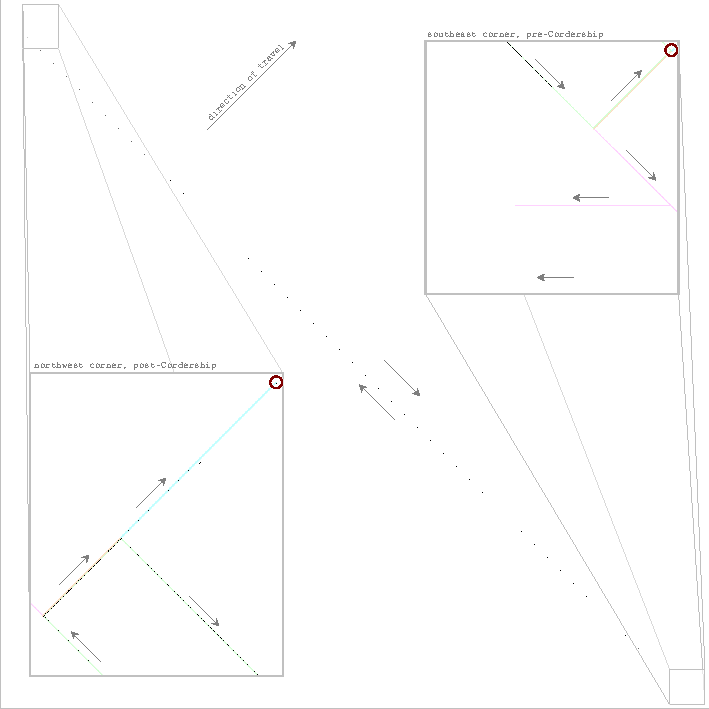
\includegraphics[width=\textwidth]{universal_construction/c256_demonoid.pdf}}
	\caption{A $c/256$ Demonoid spaceship that works by bouncing a (very long) single-channel glider recipe (highlighted in \bgbox{greenpastel}{green}) between two self-constructing ends. In the phase shown here, the recipe is about to construct a Cordership in the southeast corner (at the location circled in \bgbox{redback}{red}), which moves northeast along the path highlighted in \bgbox{aquaback}{aqua}. The single-channel glider recipe then destroys the Cordership (at the location similarly circled in the northwest corner) so as to leave behind a construction elbow. That elbow is then used to build the Snarks and Scorbie splitters necessary to repeat this process. Finally, a single glider is sent backwards as part of a Snarkbreaker, letting the single-channel glider recipe follow the path higlighted in \bgbox{magentaback}{magenta}, which is used to destroy old Snarks and Scorbie splitters that are no longer needed.}\label{fig:c256_demonoid}
\end{figure}

By waiting longer to shoot down the Cordership after it has been constructed, we can speed this Demonoid up considerably closer to the Cordership's speed of $c/12$. This design's speed limit is actually $c/14$ (not $c/12$) though, since the construction elbow must send back a backward glider as part of a Snarkbreaker once it is no longer needed, to switch the glider recipe over to the destruction elbow. That backward glider has to complete approximately half of its backward journey (i.e., it has to get back past the most-recently-constructed Scorbie splitter) before the next construction phase can begin. If the Cordership moved a total of $n$ cells before being shot down (over the course of $12n$ generations) then it will take that backward glider $4(n/2) = 2n$ generations to move backward the requisite $n/2$ cells. The total speed of the Demonoid is thus slower than $nc/(12n + 2n) = c/14$.\footnote{However, it is possible to slightly redesign this Cordership so as to avoid using a Snarkbreaker, thus pushing its not-quite-attainable speed limit up to $c/12$ from $c/14$---see the upcoming Section~\ref{sec:fast_demonoid_faster_destruction}.}


%%%%%%%%%%%%%%%%%%%%%%%%%%%%%%%%
\section{A Fast Demonoid}\label{sec:fast_demonoid}
%%%%%%%%%%%%%%%%%%%%%%%%%%%%%%%%

We now push these ideas to their absolute limit, and demonstrate how to construct Demonoids with \emph{any} rational speed below $c/4$ (rather than just speeds below $c/14$).\footnote{Recall from Theorem~\ref{thm:speed_limits} that no diagonal spaceship can go faster than $c/4$.} In order to make this possible, we have two modify the $c/256$ Demonoid from Figure~\ref{fig:c256_demonoid} in two ways:\smallskip

\begin{itemize}
	\item We have to replace the $c/12$ elbow-carrying Cordership with a $c/4$ diagonal spaceship.\smallskip
	
	\item We have to destroy any no-longer-needed circuitry without making use of Snarkbreakers\index{Snarkbreaker} (which are slow due to their usage of a long-distance backward glider on the construction lane).\smallskip
\end{itemize}

We now discuss how to implement both of these changes, so that we can construct Demonoids of essentially any speed of our choosing.


%%%%%%%%%%%%%%%%%%%%%%%%%%%%%%%%
\subsection{A Faster Elbow-Carrying Spaceship}\label{sec:fast_demonoid_elbow_carry}
%%%%%%%%%%%%%%%%%%%%%%%%%%%%%%%%

A rather large problem appears right away if we try to synthesize a $c/4$ diagional spaceship that we later shoot down from behind by gliders---those gliders cannot possibly catch up to the elbow-carrying spaceship since they travel at the same speed. To get around this problem, we instead synthesize a $c/4$ diagonal \emph{wickstretcher}, since we can burn wicks at speeds faster than $c/4$ and can thus shoot down a $c/4$ wickstretcher from behind.\index{wickstretcher}

We saw a synthesis for a $c/4$ diagonal boatstretcher\index{boatstretcher} based on the crab\index{crab} spaceship back in Exercise~\ref{exer:large_still_life_synth}, and it is fairly routine at this point to turn that glider synthesis into a unidirectional slow synthesis, and then finally into a single-channel recipe. Indeed, Figure~\ref{fig:boatstretcher_seed} shows a seed for this boatstretcher that can be triggered by just a single glider from behind\footnote{This seed was constructed and heavily optimized via a collaborative effort involving Dave Greene, Tanner Jacobi, and ConwayLife.com forums users ``Goldtiger997'' and ``toroidalet'' in July and August 2020.} (much like the single-glider seed for the Cordership from Figure~\ref{fig:2_engine_cordership_seed}). This particular seed also produces some small ash objects near the end of the boat wick (which is easily cleaned up by a few extra slow gliders---see Exercise~\ref{exer:boatstretcher_seed_slow_cleanup}), as well as a single glider that travels along the side of the boat wick, whose purpose we will see shortly.

\begin{figure}[!htb]
	\centering
	\embedlink{boatstretcher_seed}{\vcenteredhbox{\patternimg{0.121}{boatstretcher_seed_0}} \vcenteredhbox{\genarrow{553}} \vcenteredhbox{\patternimg{0.121}{boatstretcher_seed_553}}}
	
	\caption{A seed that, when hit by a single glider, produces a crab-based boatstretcher travelling in the same direction. It uses some one-time splitters and one-time turners (see Exercise~\ref{exer:boatstretcher_seed_identify}) to convert the input glider into multiple synchronized gliders that synthesize the boatstretcher.}\label{fig:boatstretcher_seed}
\end{figure}

To shoot down this boatstretcher, we fire a glider at the end of the wick (i.e., the boat that is being stretched) so as to ignite a fuse that travels faster than $c/4$, thus eventually catching up to the crab at the front and destroying it. A suitable technique for igniting a $c/3$ fuse\index{fuse} is displayed in Figure~\ref{fig:boatstretcher_shoot_down}, as is the resulting destruction of the crab boatstretcher.\footnote{There is also a common $2c/3$ fuse that can burn through this wick and destroy the crab---see Exercise~\ref{exer:boatstretcher_2c3_fuse}.} This destruction technique is why we made sure that the seed from Figure~\ref{fig:boatstretcher_seed} fires a glider next to the crab---when the fuse catches up to the crab, it just fizzles out, without actually destroying the crab itself. However, the presence of the glider changes that fizzle into an explosion, thus destroying the crab and letting us turn it back into an elbow block.

\begin{figure}[!htb]
	\centering
	\embedlink{boatstretcher_shoot_down}{\vcenteredhbox{\patternimg{0.125}{boatstretcher_shoot_down_0}} \vcenteredhbox{\genarrow{252}} \vcenteredhbox{\patternimg{0.125}{boatstretcher_shoot_down_252}} \vcenteredhbox{\genarrow{187}} \vcenteredhbox{\patternimg{0.125}{boatstretcher_shoot_down_439}}}
	
	\caption{By colliding a glider with a boat near the end of a boat wick, we can ignite a $c/3$ fuse. That $c/3$ fuse eventually catches up with the crab and glider at the front, causing them to self-destruct back into some simple ash objects (which could then be converted back into an elbow block by subsequent gliders).}\label{fig:boatstretcher_shoot_down}
\end{figure}


%%%%%%%%%%%%%%%%%%%%%%%%%%%%%%%%
\subsection{A Faster Destruction Method}\label{sec:fast_demonoid_faster_destruction}
%%%%%%%%%%%%%%%%%%%%%%%%%%%%%%%%

By making use of this wickstretcher instead of a Cordership for long-distance elbow moves, we can now construct Demonoids with speeds approaching $c/6$. However, we cannot yet get speeds arbitrarily close to $c/4$, due to the return glider that is needed for the Snarkbreaker that we discussed earlier (i.e., the same reason that the Cordership-based Demonoid of Section~\ref{sec:medium_demonoid} can reach speeds close to $c/14$, but not $c/12$). To solve this problem, we introduce another method of destroying old, no-longer-needed circuitry: by placing other still lifes nearby that facilitate their destruction.

For example, Figure~\ref{fig:snark_scorbie_seeded_destroy} illustrates how still lifes can be placed around a Snark and Scorbie splitter so that they can each be destroyed by a single glider.\footnote{Still life configurations like this that aid the self-destruction of a given pattern can be found via Simon Ekstr\"{o}m's \emph{GoL-destroy}\index{GoL-destroy} program, which is available at \httpsurl{github.com/simeksgol/GoL_destroy}.} Importantly, these still lifes do not interfere with the usual function of the circuit (which is to either reflect or duplicate a glider).

The circuit-destroying glider comes from the same direction as the usual input glider, but on a different lane. When destruction is complete, a glider is released, aimed at the next piece of circuitry that is due to be destroyed, with exactly the correct timing relative to the final recipe gliders. This allows circuit destruction to be triggered immediately, without having to wait for a return glider from far away as in a Snarkbreaker.

\begin{figure}[!htb]
	\centering
	\begin{subfigure}{0.455\textwidth}
		\centering
		\embedlink{snark_seeded_destroy}{\vcenteredhbox{\patternimg{0.110419214}{snark_seeded_destroy_0}} \vcenteredhbox{\genarrow{240}} \vcenteredhbox{\patternimg{0.110419214}{snark_seeded_destroy_240}}}
		\caption{A Snark, seeded with 3 extra still lifes, being destroyed by a single glider.}
		\label{fig:snark_seeded_destroy}
	\end{subfigure} \hfill % 
	\begin{subfigure}{0.505\textwidth}
		\centering
		\embedlink{scorbie_splitter_seeded_destroy}{\vcenteredhbox{\patternimg{0.094}{scorbie_splitter_seeded_destroy_0}} \vcenteredhbox{\genarrow{551}} \vcenteredhbox{\patternimg{0.094}{scorbie_splitter_seeded_destroy_551}}}
		\caption{A Scorbie splitter, seeded with 8 extra still lifes, being destroyed by a single glider.}
		\label{fig:scorbie_splitter_seeded_destroy}
	\end{subfigure}
	\caption{Additional still lifes (displayed in \bgbox{redback}{red}) can be placed near a circuit so as to make it simpler to destroy, without affecting its functionality. Here we use (a) 3 extra still lifes to turn a Snark into a one-time turner, and (b) 8 extra still lifes to turn a Scorbie splitter into a one-time splitter.}\label{fig:snark_scorbie_seeded_destroy}
\end{figure}

It's important to notice that these destruction recipes produce output gliders, so we don't need to generate the destruction-triggering gliders via single-channel recipes at all. Instead, we can just use a single glider that follows along behind (but slightly offset from) the single-channel recipe. This cleanup glider triggers the destruction of every single piece of circuitry in the Demonoid once it is no longer needed, in a continuous chain reaction. After one piece of circuitry is cleaned up, the glider is reflected toward the next piece of circuitry that needs cleaning up, and so on. Again, the timing has to be carefully controlled so that the cleanup glider neither catches up to the recipe nor falls behind it.



%%%%%%%%%%%%%%%%%%%%%%%%%%%%%%%%
\subsection{The Speed Demonoid Itself}\label{sec:speed_demonoid}\index{Speed Demonoid}
%%%%%%%%%%%%%%%%%%%%%%%%%%%%%%%%

Now that we have faster elbow-moving and circuit-destroying techniques, we can build a much faster Demonoid, appropriately named the \textbf{Speed Demonoid}.\footnote{Constructed by Pavel Grankovskiy in September 2020.} The general layout of this Demonoid is very similar to that of the other Demonoids that we have seen---it is mostly made up of its single-channel glider recipe, which creates Snarks and Scorbie splitters that it zig-zags back and forth between.

The only additional wrinkle that we add to this Demonoid design is that we use the crab as a \emph{double} boatstretcher instead of just as a single boatstretcher. That is, we will have the crab create and stretch two boat wicks, as illustrated in Figure~\ref{fig:double_boatstretcher_shoot_down}. The reason for making this change is that we want to use the crab to create two construction elbows, not just one---an elbow for making the next Scorbie splitter, and another elbow for making the next Snark. The two boat wicks can be burned independently so as to create those elbow blocks whenever we like (though we must be careful that the crab is only destroyed by the second fuse, not the first).

\begin{figure}[!htb]
	\centering
	\embedlink{double_boatstretcher_shoot_down}{\vcenteredhbox{\patternimg{0.125}{double_boatstretcher_shoot_down_0}} \vcenteredhbox{\genarrow{343}} \vcenteredhbox{\patternimg{0.125}{double_boatstretcher_shoot_down_343}}}
	
	\caption{A double boatstretcher that can have its two wicks ignited independently, allowing the crab two carry two construction elbows instead of just one. Here, the first fuse (highlighted in \bgbox{aquaback}{aqua}) creates a small explosion, without hurting the crab, that the nearby glider helps turn into the first elbow. The second fuse (highlighted in \bgbox{magentaback}{magenta}) then destroys the crab, and the nearby glider helps turn it into the second elbow, as in Figure~\ref{fig:boatstretcher_shoot_down}.}\label{fig:double_boatstretcher_shoot_down}
\end{figure}

We similarly needed to make two construction elbows in each of our previous Demonoids. In the slow Demonoid from Figure~\ref{fig:slow_demonoid}, we first pushed the construction elbow to the correct location to build the next Scorbie splitter, and then once it was built we pushed the construction elbow forward again to the correct location to build the next Snark. In the $c/256$ Demonoid from Figure~\ref{fig:c256_demonoid}, the Cordership was shot down into an elbow at the location of the next Snark, and then a backward glider was shot back to create an elbow at the location of the next Scorbie splitter (alternatively, we could have used two Corderships). We could use similar tricks in this Speed Demonoid, but a double boatstretcher is a bit faster and more elegant than two single boatstretchers.

Rather than using zero-degree recipes to build the gliders that ignite the boat $c/3$ boat fuses, it will be slightly more efficient to place two isolated gliders on their own lanes, away from the single-channel recipe, so as trigger the ignitions. We can redirect these gliders, which we refer to as \texttt{TRIGGER1} and \texttt{TRIGGER2},\index{TRIGGER1}\index{TRIGGER2} around the same path as the single-channel recipe via one-time turners and one-time splitters (rather than Snarks and Scorbie splitters). Furthermore, since the Snark and Scorbie splitter destruction technique of Figure~\ref{fig:snark_scorbie_seeded_destroy} turns those circuits into one-time-turners and splitters, respectively, the \texttt{TRIGGER2} glider can naturally serve a secondary role as the one that destroys no-longer-needed Snarks and Scorbie splitters.

Putting all of this together finally gives us a completed Speed Demonoid, which is displayed in Figure~\ref{fig:speed_demonoid}.

\begin{figure}[!htbp]
	\centering
	\embedlink{speed_demonoid}{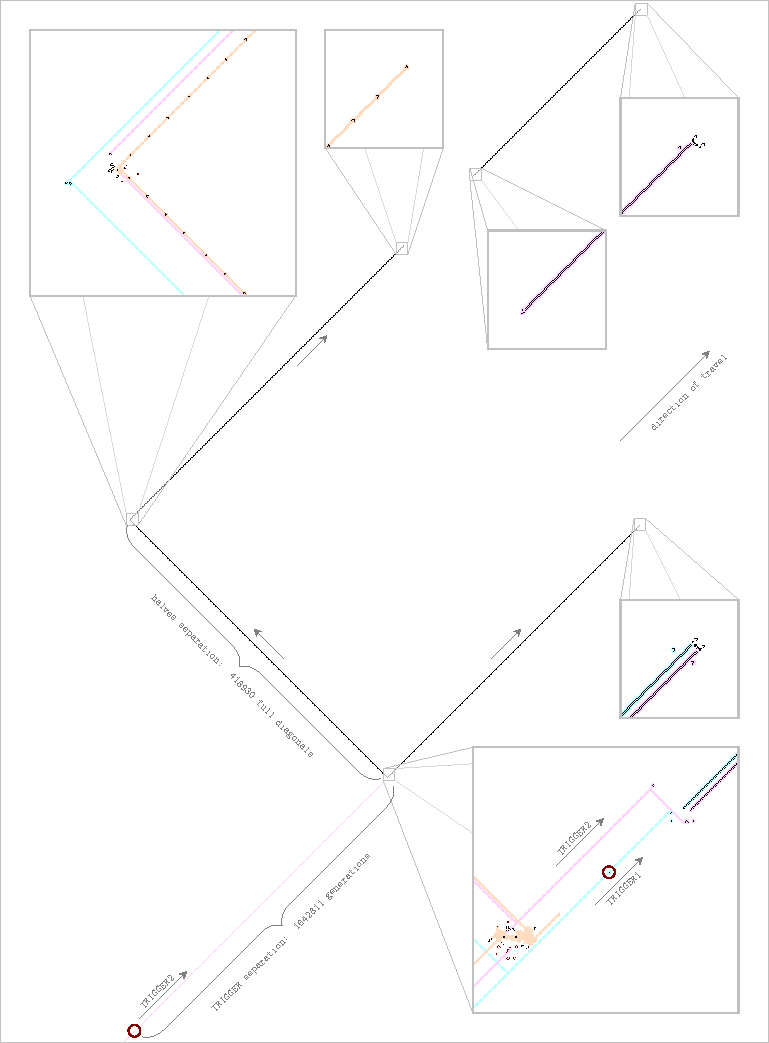
\includegraphics[width=\textwidth]{universal_construction/speed_demonoid.pdf}}
	\caption{A Speed Demonoid spaceship that moves $3{\thousep}285{\thousep}622$ cells diagonally every $16{\thousep}493{\thousep}928$ generations, for a speed of $1642811c/8246964 \approx 0.1992c$. The single-channel glider recipe (whose path is highlighted in \bgbox{orangeback2}{orange}) constructs Snarks, Scorbie splitters, and crab-based double boatstretchers. The two \texttt{TRIGGER} gliders (circled in \bgbox{redback}{red} and highlighted in \bgbox{aquaback}{aqua} and \bgbox{magentaback}{magenta}, respectively) each ignite one of the fuses behind the boatstretcher, and \texttt{TRIGGER2} also destroys no-longer-needed Snarks and Scorbie splitters.}\label{fig:speed_demonoid}
\end{figure}


%%%%%%%%%%%%%%%%%%%%%%%%%%%%%%%%
\subsection{Adjusting the Speed Demonoid}\label{sec:speed_demonoid_adjust}
%%%%%%%%%%%%%%%%%%%%%%%%%%%%%%%%

Now that we have constructed a single Speed Demonoid, it is straightforward to adjust its speed, even by hand. In the Speed Demonoid of Figure~\ref{fig:speed_demonoid}, there are two parameters that we are free to adjust:\smallskip

\begin{itemize}
	\item[1)] The first parameter is the number of full diagonals separating the two mirror-image halves of the Demonoid, which we denote by $m$. We used a separation of $m = 418{\thousep}930$ full diagonals in Figure~\ref{fig:speed_demonoid}, and increasing $m$ has the usual effect of increasing the Demonoid's period by $8$~generations, without changing how far it moves over the course of its period.\smallskip
	
	\item[2)] The second parameter is the number of generations between the isolated \texttt{TRIGGER1} and \texttt{TRIGGER2} gliders, which we denote by $n$. We used a separation of $n = 1{\thousep}642{\thousep}811$~generations in Figure~\ref{fig:speed_demonoid}, and we have to be slightly careful about increasing it. The separation between the two trigger gliders determines how far apart each Snark will be from the subsequent Scorbie splitter, so to keep the two halves of the Demonoid lined up, we need to similarly adjust the spacing between each Snark and the \emph{preceding} Scorbie splitter. Thus if we increase the trigger separation $n$, we also have to move both trigger gliders back by that same amount.\footnote{In other words, to separate the trigger gliders by $k$ more generations, we should move \texttt{TRIGGER1} and \texttt{TRIGGER2} back by $k$ and $2k$~generations, respectively (not $0$ and $k$~generations, respectively).}\smallskip
\end{itemize}

The trigger gap $n = 1{\thousep}642{\thousep}811$ that we used in the Speed Demonoid of Figure~\ref{fig:speed_demonoid} is minimal---any smaller gap between the two trigger gliders would result in either \texttt{TRIGGER1} attempting to light the fuse while some of the mechanism is still under construction, or \texttt{TRIGGER2} crashing into a Snark while it's still under construction. Similarly, the value of $n+m = 2{\thousep}061{\thousep}741$ (which measures the total length of the track along which the single-channel recipe travels) that we used in Figure~\ref{fig:speed_demonoid} is also minimal---any smaller value of $n+m$ would result in the single-channel recipe trying to use a Snark before it is done being built.

While we cannot decrease $n$ or $n+m$,\footnote{However, we can decrease $m$ (the width of the Speed Demonoid) as long as we increase $n$ by the same amount or more.} we are free to \emph{increase} $n$ and $m$ as much as we like, resulting in larger and larger Speed Demonoids. After adjusting the values of $n$ and $m$ to our liking, the resulting Speed Demonoid's speed will be
\[
	\frac{2nc}{8n + 8m} = \left(\frac{n}{n+m}\right)\frac{c}{4}.
\]

Every rational number between $0$ and $1$ can be written in the form $n/(n+m)$ for some integers $m,n > 0$, simply by first choosing $n$ to get whatever numerator we want, and then choosing $m$ to get whatever denominator we want. Furthermore, since $n/(n+m) = (kn)/(kn+km)$ for all $k > 0$, we can choose $m$ and $n$ to be as large as we like. In particular, we can choose $n \geq 1{\thousep}642{\thousep}811$ and $n+m \geq 2{\thousep}061{\thousep}741$ so that the resulting Speed Demonoid is actually constructible.

For example, to build a $3c/14$ Speed Demonoid, we want $n/(n+m) = 4(3/14) = 12/14$, so we could first choose $n = 12$ and then $m = 2$ (so that $n+m = 14$). However, these values of $n$ and $m$ are much too small for us to actually be able to build a Speed Demonoid with these parameters (we cannot separate the trigger gliders by just $n = 12$ generations, for example, without components crashing into each other), so we scale them up. That is, we replace $n$ and $m$ by $\widetilde{n} = kn$ and $\widetilde{m} = km$, respectively, where $k$ is an integer chosen so that $kn \geq 1{\thousep}642{\thousep}811$ and $k(n+m) \geq 2{\thousep}061{\thousep}741$.\footnote{In other words, $k \geq \max\{ \lceil 1{\thousep}642{\thousep}811/n \rceil, \lceil 2{\thousep}061{\thousep}741/(n+m) \rceil \}$.} In this case, $k = 147{\thousep}268$ works, which gives $\widetilde{n} = 12 \times 147{\thousep}268 = 1{\thousep}767{\thousep}216$ and $\widetilde{m} = 2 \times 147{\thousep}268 = 294{\thousep}536$ (see Exercise~\ref{exer:3c14_speed_demonoid}).

This procedure works in general, and shows that Speed Demonoids can be adjusted to have any rational speed that is slower than $c/4$. In fact, there is a computer script\footnote{Available for download at \httpsurl{conwaylife.com/forums/viewtopic.php?p=105167\#p105167}.} that carries out this adjustment automatically, and can construct a Speed Demonoid of any desired (rational, slower than $c/4$) speed.


% Maybe todo: it would be nice, but perhaps not necessary, to have the reverse caber-tosser in the book. If we do that though, it has to be its own proper section. I cannot imagine trying to cram it into the notes/history section of Ch11 like I originally intended to do.
% Maybe simplest visualization of the RCT is here?: https://www.conwaylife.com/forums/viewtopic.php?p=104484#p104586
%%%%%%%%%%%%%%%%%%%%%%%%%%%%%%%%
\section{Notes and Historical Remarks}\label{sec:universal_construction_history}
%%%%%%%%%%%%%%%%%%%%%%%%%%%%%%%%

While universal construction has been known to be possible since the early days of Life \cite{Wain74,BCG82}, it took almost 40 more years of work for the Life community to streamline it to the point that it is actually small and fast enough to watch in action.

Paul Chapman and Dave Greene built the first universal constructor in 2004 (see Figure~\ref{fig:chapman_greene_constructor}), and it made use of the exact same construction arm that we saw in Figure~\ref{fig:construction_arm}. However, instead of encoding the \texttt{PULL}, \texttt{PUSH}, \texttt{FIRE WHITE}, and \texttt{FIRE BLACK} commands directly in the input stream of gliders (as was done with the Gemini spaceship of Figure~\ref{fig:gemini}), they were stored in unary as boats that were separated via sequences of zero, one, two, or three blocks. This resulted in an average of two and a half bits of static storage being used to encode two bits' worth of information---rather inefficient, but it was only intended as an initial prototype.

% https://comp.theory.cell-automata.narkive.com/Z17teVRa/a-prototype-programmable-universal-constructor-for-conway-s-life
\begin{figure}[!htbp]
	\centering
	\embedlink{chapman_greene_constructor}{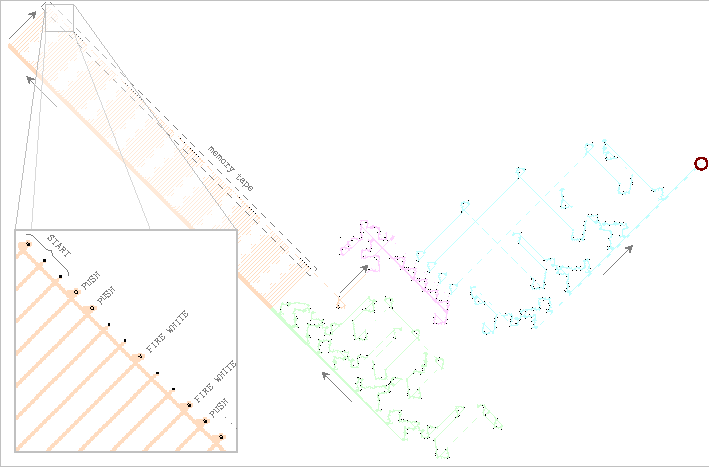
\includegraphics[width=\textwidth]{universal_construction/chapman_greene_constructor.pdf}}
	\caption{A universal constructor that was built by Paul Chapman and Dave Greene in 2004. The conduit highlighted in \bgbox{greenpastel}{green} fires $10$-glider salvos toward the memory tape that is highlighted in \bgbox{orangeback2}{orange}. Those salvos read the memory tape by either detecting a boat and sending a glider back, or detecting a block and sending nothing back. If a boat was detected, the returned glider is fed into the \bgbox{magentaback}{magenta} conduit, which keeps track of how many generations passed between receiving input gliders (i.e., how many blocks there were between boats on the memory tape). That generation gap determines which of four lanes is used to feed into the construction arm that is highlighted in \bgbox{aquaback}{aqua}, and thus which of the four construction operations is performed.}\label{fig:chapman_greene_constructor}
\end{figure}

The next major development in this area came in 2010 with Adam P.~Goucher's universal computer-constructor. While we have not explicitly explored the ``constructor'' part of this device, it uses the same construction arm that we have already seen, in conjunction with the binary register from Section~\ref{sec:binary_register} for storing the construction instructions. This binary storage is more efficient than the unary storage of the Chapman--Greene prototype, and the fact that it comes as part of a programmable computer makes it more straightforward to actually make use of.

Both the Chapman--Greene constructor prototype, as well as the Goucher constructor, produced their output unidirectional slow glider salvos by reading a tape consisting of still lifes that represented sequences of glider-firing operations. The idea of encoding information via static objects like this was deeply ingrained in the Life community at the time, likely as a result of how information is similarly stored in actual computers. However, the sudden appearance of the Gemini in 2010 showed that this method of storing data was just silly. Obviously (with hindsight), if you want to build some kind of memory storage system for a bunch of spacings between gliders, you just store a bunch of moving gliders at the spacing you want---there is no need to encode anything at all.

That one insight allowed Andrew J.~Wade, who was a complete newcomer to the Life community, to build the first ever oblique and/or self-constructing spaceship, even using extraordinarily sub-optimal components. The Chapman--Greene prototype universal constructor was a first proof of concept, not really intended to be used anywhere since it could straightforwardly be made so much smaller. But Wade wasn't a stable circuitry expert, so he just used what was available: the Gemini spaceship included not just one, but three complete copies of the prototype construction arm, almost completely unmodified. All he did was throw away the hopelessly inefficient static storage system and substitute something better.

The Gemini's completion, and its accompanying philosophy of storing information in glider streams instead of sequences of still lifes, marked the start of a new era of Life construction. In addition to the Geminoids and Demonoids that we saw in this chapter, a flood of other self-constructing spaceships and bizarre patterns based on universal construction were built in the 2010s. Some of the more notable examples include:\smallskip

\begin{itemize}
	\item In October 2010, Paul Tooke constructed numerous \textbf{pianola breeders}:\index{pianola breeders} breeders that work by using universal constructors to synthesize objects that then synthesize other objects.\index{breeder} Because of the flexibility of universal construction, these breeders could be configured to behave in extremely unusual ways. For example, one of these breeders consists of a stationary object (a pair of universal constructors) that synthesizes stationary objects (slide guns), which then synthesize more stationary objects (lines of beehives).\footnote{See \httpsurl{conwaylife.com/wiki/Pianola_breeder}, and contrast this with the other breeders that we have seen, which all require some of the synthesized objects to move.}\smallskip
	
	\item In November 2013, Dave Greene built a pattern called a \textbf{linear propagator}\footnote{See \httpsurl{conwaylife.com/wiki/Linear_propagator}.}\index{linear propagator} that repeatedly makes copies of itself---something that had been known to be possible since the early 1970s, but had eluded construction for the intervening four decades.\smallskip
	
	\item In August 2014, Dave Greene constructed a pattern that grows outward in a spiral fashion by laying ever-expanding tracks around itself. The original version of this pattern had a bounding box with side length of approximately $1.6$~million cells, but has since between reduced to approximately $2{\thousep}000$ cells (see Figure~\ref{fig:spiral_growth}\index{spiral growth} and Exercise~\ref{exer:snark_spiral_weld}).\smallskip
	
	\item In November 2015, Chris Cain and Dave Greene completed the first Demonoid, which used somewhat more complicated circuitry than the Demonoids that we investigated in this chapter. Most notably, it used pairs of gliders separated by $10$hd to implement slow glider syntheses instead of single-channel glider recipes, which doubled the amount of circuitry that had to be constructed at each end.\smallskip
	
	\item In June 2017, Dave Greene constructed an \textbf{Orthogonoid}\index{Orthogonoid} spaceship,\footnote{See \httpsurl{conwaylife.com/wiki/Orthogonoid}.} which works similarly to Demonoids, except uses middleweight spaceships (instead of gliders) to achieve a slow orthogonal (instead of diagonal) speed of travel. Adam P.~Goucher then helped build faster Orthogonoids with speeds up to $65536c/951573 \approx 0.06887c$ in October 2018.\smallskip
	
	\item In December 2018, Chris Cain completed a\index{camelship} \textbf{camelship}\footnote{See \httpsurl{conwaylife.com/wiki/Camelship}.} by modifying an earlier \textbf{volatility~1 oscillator}\footnote{See \httpsurl{conwaylife.com/wiki/Volatility}.} design. The oscillator ensures that all its cells oscillate at the pattern's full period, by using single-channel glider recipes to destroy then rebuild its own circuitry. The camelship consists of a very similar single-channel signal loop, but the circuit reconstruction happens at a $(3,1)$ offset.\smallskip
	
	\item In April 2019, Michael Simkin constructed \textbf{Remini},\footnote{Short for \textbf{R}etro G\textbf{emini}, in reference to the fact that it uses old-style p30 circuitry instead of more modern stable circuitry. See \httpsurl{conwaylife.com/wiki/Remini}.}\index{Remini} an oblique self-constructing puffer that is designed like a single-channel version of the Gemini, but which uses period~$30$ circuitry to perform the glider reflections and duplications instead of stable circuitry. The tricky thing about constructing this device was the fact that the single-channel recipe has to align with the p$30$ circuitry, so the only timing gaps that are allowed are multiples of $30$.\smallskip
	
	\item In August 2021, ConwayLife.com forums user ``Goldtiger997'' constructed a \textbf{spaceship made of spaceships}---a\index{spaceship made of spaceships} spaceship that, in one of its phases, consists only of $144{\thousep}221$ gliders. They also constructed a \textbf{reflectorless rotating oscillator}---an\index{reflectorless rotating oscillator} oscillator that rotates around a point in the Life plane without the help of any fixed circuitry like Snarks. We discuss these types of patterns in more depth in Section~\ref{sec:other_ca_rules}.\smallskip
\end{itemize}

The development of single-channel glider synthesis mostly took place in 2017, when another relative newcomer, Simon Ekstr{\"o}m, cavalierly disregarded accumulated prejudices from the previous decade, tried a search, and found that it worked.\footnote{This is not unlike Wade's construction of the Gemini in 2010, or when ConwayLife.com forums user ``zdr'' found the copperhead spaceship in 2016. In all of these cases, a newcomer simply looked where the members of the Life community thought there wasn't anything to find.} It was already known in 2015 how to emulate arbitrary glider synthesis via gliders on a single lane, but Ekstr{\"o}m was the first to show that it is possible even when the gliders are far enough apart from each other that they can be fed through standard components like Snarks and syringes.


% Put figure down below clearpage to force exercises header onto same page as it. Can remove if/when page breaks adjust. (currently removed)

\begin{figure}[!htb]
	\centering
	\embedlink{spiral_growth}{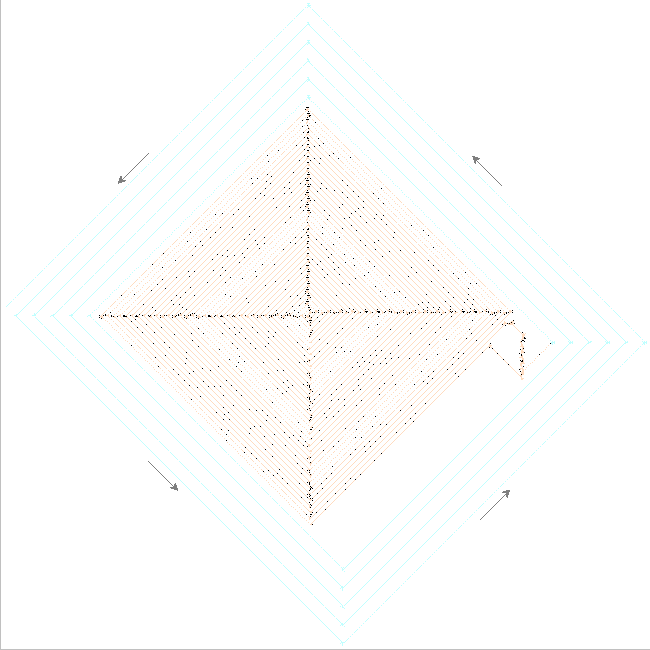
\includegraphics[width=\textwidth]{universal_construction/spiral_growth.pdf}}
	\caption{A spiral growth pattern that was constructed by Dave Greene in June 2017. A single-channel recipe that is primarily made up of a Snarkmaker bounces around the diamond-shaped track highlighted track in \bgbox{orangeback2}{orange}, creating Snarks that extend the track as indicated in \bgbox{aquaback}{aqua}.}\label{fig:spiral_growth}
\end{figure}

%\clearpage % Put "Exercises" header at the top of the next page instead of the bottom of this page


%%%%%%%%%%%%%%%%%%%%%%%%%%%%%%%%%
\section*{Exercises \hfill \normalfont\textsf{\small solutions to starred exercises on \hyperlink{solutions_universal_construction}{page \pageref{solutions_universal_construction}}}}
\label{sec:universal_construction_exercises}
\addcontentsline{toc}{section}{Exercises}
\vspace*{-0.4cm}\hrulefill\vspace*{-0.3cm}\footnotesize\begin{multicols}{2}\vspace*{-0.4cm}\raggedcolumns\interlinepenalty=10000
	\setlength{\parskip}{0pt}
	%%%%%%%%%%%%%%%%%%%%%%%%%%%%%%%%%
	
	\begin{problem}\label{exer:rebuild_construction_arm} \probdiff{3}
		Rebuild the construction arm from Figure~\ref{fig:construction_arm} via modern components like Snarks and syringes.
	\end{problem}
	
	
	\mfilbreak
	
	
	\begin{problem}\label{exer:construction_arm_lanes_timed}
		The construction arm of Figure~\ref{fig:construction_arm} requires two synchronized input gliders to trigger each of the \texttt{PUSH}, \texttt{FIRE WHITE}, and \texttt{FIRE BLACK} operations---one to create the frontmost pair of gliders via the \texttt{PULL} input, and one to create the additional glider(s) via one of the other three inputs.\smallskip
		
		\begin{enumerate}[label=\bf\color{ocre}(\alph*)]
			\item \probdiff{2} Find the correct timing for the pair of input gliders to trigger each of the \texttt{PUSH}, \texttt{FIRE WHITE}, and \texttt{FIRE BLACK} operations.
			
			\item \probdiff{3} Add additional Herschel conduits to that arm (or the one from Exercise~\ref{exer:rebuild_construction_arm}) so that each of the four operations can be triggered by just a single input glider.
		\end{enumerate}
	\end{problem}
	
	
	\mfilbreak
	
	
	\begin{problem}\label{exer:construction_arm_fire_white_different} \probdiff{1}
		The arrangement of two gliders that the \texttt{FIRE WHITE} circuit in Figure~\ref{fig:construction_arm} makes is slightly different than the pair of \texttt{FIRE WHITE} gliders highlighted in green in Figure~\ref{fig:gemini_fire_white}. Why is this not a problem?
	\end{problem}
	% SOLUTION: The first 3 gliders create a one-time-turner boat. It doesn't matter when the fourth glider hits that boat, as long as it is one the right lane.
	
	
	\mfilbreak
	
	
	\begin{problem}\label{exer:mwss_universal_constructor_turn_into_gun} \probdiff{3}
		The pattern in Figure~\ref{fig:mwss_universal_constructor} uses two universal constructors to synthesize a middleweight spaceship.\smallskip
		
		\begin{enumerate}[label=\bf\color{ocre}(\alph*)]
			\item Add a loop gun to each of the 8 input lanes, so that universal constructor \emph{repeatedly} constructs middleweight spaceships.
			
			\item Adjust the input glider recipes so that each middleweight spaceship is produced on the same lane as the previous one (thus making this pattern a middleweight spaceship gun).
			% Solution: Add some PULLs on each lane after the final FIRE BLACK
		\end{enumerate}
	\end{problem}
	
	
	\mfilbreak
	
	
	\begin{problem}\label{exer:mwss_universal_constructor_turn_into_other}
		Adjust the input glider sequences for the pattern from Figure~\ref{fig:mwss_universal_constructor} so that instead of constructing an MWSS, it constructs...\smallskip
		
		\begin{enumerate}[label=\bf\color{ocre}(\alph*)]
			\item \probdiff{3} a lightweight spaceship,
			
			\item \probdiff{3} a line of blocks (of any slope and spacing of your choosing), and
			
			\item \probdiff{5} a $2$-engine Cordership.
			
			[Hint: You can use the $2$-direction slow synthesis from Figure~\ref{fig:armless_cordership_gun}.]
		\end{enumerate}
	\end{problem}
	
	
	\mfilbreak
	
	
	\begin{problemstar}\label{exer:gemini_unhighlighted_reflectors} \probdiff{2}
		The two zoom boxes in Figure~\ref{fig:gemini} each have two rows of unhighlighted reflectors that never reflect a single glider. What is their purpose?
	\end{problemstar}
	
	
	\mfilbreak
	
	
	\begin{problem}\label{exer:gemini_which_lane_operations} \probdiff{3}
		The 12 glider lanes in the Gemini spaceship from Figure~\ref{fig:gemini} each implement one of the 4 basic operations from Figure~\ref{fig:gemini_glider_operations} (i.e., \texttt{PULL}, \texttt{PUSH}, \texttt{FIRE WHITE}, and \texttt{FIRE BLACK}). Determine which lanes implement which of those operations.
	\end{problem}
	
	
	\mfilbreak
	
	
	\begin{problem}\label{exer:gemini_separate_ends_slow} \probdiff{3}
		Move the two identical ends of the Gemini spaceship farther apart, so as to create a spaceship that travels slower than $(1024,5120)c/50000000$.
	\end{problem}
	
	
	\mfilbreak
	
	
	\begin{problemstar}\label{exer:squeeze_gemini_how_far} \probdiff{4}
		By moving the two identical ends of the Gemini spaceship closer together, we can make it slightly faster.\smallskip
		
		\begin{enumerate}[label=\bf\color{ocre}(\alph*)]
			\item Move the ends $1$~full diagonal closer together. What is the speed of the resulting spaceship?
			
			\item How many full diagonals closer together can the ends be moved without causing the Gemini to self-destruct? What is the speed of the resulting spaceship?
			% Explicitly built at https://www.conwaylife.com/forums/viewtopic.php?f=2&t=406#p2564
		\end{enumerate}
	\end{problemstar}
	
	
	\mfilbreak
	
	
	\begin{problemstar}\label{exer:gemini_slope_n_fixed} \probdiff{3}
		The slope-$2$ Geminoid from Figure~\ref{fig:geminoid_knightship} was created by just adding additional \texttt{PUSH} operations to the northwest construction elbow (i.e., we increased the value that we called ``$m$'' in that section, while leaving ``$n$'' fixed at $n = 2{\thousep}048$). What Geminoid slopes are attainable by making this type of change to Gemini? That is, what slopes can be attained by increasing $m$, but not changing $n$?
	\end{problemstar}
	
	
	\mfilbreak
	
	
	\begin{problem}\label{exer:gemini_slope_3}
		Recall that the Gemini itself travels at slope $5$, and the Geminoid knightship travels at slope $2$.\smallskip
		
		\begin{enumerate}[label=\bf\color{ocre}(\alph*)]
			\item \probdiff{2} To create a Geminoid that travels at a slope of $3$, how many \texttt{PUSH} operations should we add to the path of the northwest construction elbow?
			% SOLUTION: 1024, which gives a displacement in that direction of m = 4096 instead of 3072.
			
			\item \probdiff{5} Construct a Geminoid that travels at a slope of $3$.
		\end{enumerate} Gemini)
	\end{problem}
	
	
	\mfilbreak
	
	
	% TODO: Give solution? Easy one to give solutions to.
	\begin{problem}\label{exer:move_single_channel_elbow} \probdiff{2}
		String together multiple elbow-moving single-channel glider recipes from Table~\ref{tab:single_lane_elbow_movers} so as to make a recipe that moves the elbow forward by exactly...\smallskip
		
		\begin{enumerate}[label=\bf\color{ocre}(\alph*)]
			\item $11$ half diagonals,
			
			\item $-25$ half diagonals, and
			
			\item $38$ half diagonals.
		\end{enumerate}
	\end{problem}
	
	
	\mfilbreak
	
	
	% TODO: Give solution? Easy one to give solutions to.
	\begin{problem}\label{exer:single_channel_90_degree_fire} \probdiff{3}
		String together multiple single-channel glider recipes from Tables~\ref{tab:single_lane_90deg_glider_timings} and~\ref{tab:single_lane_elbow_movers} so as to fire a single glider on output lane...\smallskip
		
		\begin{enumerate}[label=\bf\color{ocre}(\alph*)]
			\item $3x$,
			
			\item $0i$, and
			
			\item $15x$.
		\end{enumerate}
	\end{problem}
	
	
	\mfilbreak
	
	
	\begin{problem}\label{exer:block_pull_pond} \probdiff{2}
		The single-channel elbow-pulling sequence displayed in Figure~\ref{fig:0_degree_block_pull} turns an elbow block into a pond (rather than another block). Why is this not a problem?
	\end{problem}
	% Pond acts as an elbow in the same way (also explodes into a pi-heptomino)
	
	
	\mfilbreak
	
	
	\begin{problemstar}\label{exer:single_lane_glider_final_glider_explain} \probdiff{2}
		The 185-glider single-lane sequence illustrated in Figure~\ref{fig:90_degree_block_move} makes use of two copies of the glider sequence that moves the elbow forward by $10$ half-diagonals. In the first sequence the final glider arrives after 90~generations, whereas in the second sequence it arrives after 91~generations. Explain the reason for this discrepancy---why can't the final glider in the second sequence also arrive after just 90~generations?
	\end{problemstar}
	
	
	\mfilbreak
	
	
	\begin{problem}\label{exer:push_elbow_longer} \probdiff{2}
		The following single-lane glider recipe moves the elbow block:
		\begin{align*}
		& \text{\texttt{\footnotesize 109, 91, 93, 91, 145, 215, 106, 90, 90,}} \\
		& \text{\texttt{\footnotesize~91, 91, 174, 90, 158, 90, 90, 90, 91,}} \\
		& \text{\texttt{\footnotesize~~~~~~~~137, 90, 91, 127, {\color{gray}(90)}.}}
		\end{align*}
		
		\begin{enumerate}[label=\bf\color{ocre}(\alph*)]
			\item How many half-diagonals (and in which direction) does this sequence move the elbow?
			% SOLUTION: 20, forward
			
			\item Use this 23-glider sequence to rebuild the 185-glider sequence from Figure~\ref{fig:90_degree_block_move} to be at least $15$~gliders shorter, while still performing the same task (i.e., building a hand block and then moving it south by $11$~cells).
			% SOLUTION: Replace the pair of 10hd moves with this single 20hd move.
		\end{enumerate}
	\end{problem}
	
	
	\mfilbreak
	
	
	\begin{problemstar}\label{exer:0degree_hand_move} \probdiff{1}
		What is the ``move'' value of the zero-degree hand-making glider sequence from Figure~\ref{fig:0degree_hand} (i.e., how many half-diagonals is the elbow block moved)?
	\end{problemstar}
	
	
	\mfilbreak
	
	
	\begin{problem}\label{exer:exercise_hwss_slow_salvo} \probdiff{3}
		An 8-glider unidirectional slow salvo that synthesizes a heavyweight spaceship\footnote{Found by Adam P.~Goucher in December 2016.} is displayed below:
		
		\noindent\begin{center}
			\patternimglink{0.112}{exercise_hwss_slow_salvo}
		\end{center}
		
		\begin{enumerate}[label=\bf\color{ocre}(\alph*)]
			\item Use the recipes of Tables~\ref{tab:single_lane_90deg_glider_timings} and~\ref{tab:single_lane_elbow_movers} to emulate this slow salvo via a single-channel glider recipe and a 90-degree elbow.
			
			\item Use the recipes of Table~\ref{tab:single_lane_0deg_glider_timings} to emulate this slow salvo via a single-channel glider recipe and a zero-degree elbow.
		\end{enumerate}
	\end{problem}
	
	
	\mfilbreak
	
	
	\begin{problem}\label{exer:snark_slow_salvo_pieces} \probdiff{2}
		The $95$-glider slow salvo synthesis of a Snark from Figure~\ref{fig:snark_slow_salvo} is an incremental synthesis. Break it down into steps like we did with the $94$-glider synthesis from Figure~\ref{fig:17_cell_synthesis}.
	\end{problem}
	
	
	\mfilbreak
	
	
	\begin{problem}\label{exer:cordership_slow_salvo_from_single_channel} \probdiff{3}
		Extract a $112$-glider unidirectional slow-salvo synthesis of a $2$-engine Cordership from the $2{\thousep}393$-glider single-channel recipe that is provided in Appendix~\ref{sec:appendix_cordership_maker}.
	\end{problem}
	
	
	\mfilbreak
	
	
	\begin{problemstar}\label{exer:scorbie_splitter_slow_salvo} \probdiff{3}
		Extract a unidirectional slow-salvo synthesis of a Scorbie splitter from the $4{\thousep}006$-glider single-channel recipe that is provided in Appendix~\ref{sec:appendix_scorbie_splitter_maker}. How many gliders does this slow salvo have?
	\end{problemstar}
	
	
	\mfilbreak
	
	
	\begin{problem}\label{exer:scorbie_splitter_zero_degree} \probdiff{3}
		Use slsparse (\httpsurl{conwaylife.com/wiki/Slsparse}) to create a single-channel glider recipe that synthesizes a Scorbie splitter in the following orientation, starting with a zero-degree elbow block in the location indicated at the top-center:
		
		\noindent\begin{center}
			\patternimglink{0.11}{exercise_single_channel_scorbie_splitter}
		\end{center}
	\end{problem}
	
	
	\mfilbreak
	
	
	\begin{problemstar}\label{exer:slow_demonoid_adjust} \probdiff{2}
		The bounding box of the slow Demonoid from Figure~\ref{fig:slow_demonoid} can be decreased considerably just by moving its two stabilizing ends closer together, and doing so also reduces its period and increases its speed.
		
		Adjust that Demonoid so that the longest side of its bounding box is no more than $200{\thousep}000$ cells long. What are its period and speed after you make this adjustment?
	\end{problemstar}
	
	
	
	\mfilbreak
	
	
	\begin{problem}\label{exer:gemini_why_any_slope_demonoid_fixed} \probdiff{2}
		Recall that the Gemini can be modified to travel in essentially any rational direction, whereas Demonoids can only travel diagonally with slope~1. Explain why---what key aspect of their designs differs?
	\end{problem}
	% Solution: because gemini's ends are exact copies of each other, whereas demonoid ends are glide-reflections.
	
	
	\mfilbreak
	
	
	\begin{problem}\label{exer:snark_scorbie_splitter_xwss_destroy} \probdiff{3}
		Recall the $461$-glider single-channel recipe from Appendix~\ref{sec:appendix_scorbie_splitter_destroyer} that produces the $6$-xWSS slow salvo of Figure~\ref{fig:scorbie_splitter_xwss_destroy} for destroying a Scorbie splitter.
		
		\begin{enumerate}[label=\bf\color{ocre}(\alph*)]
			\item Separate this single-channel recipe into smaller recipes that (i) move the elbow, (ii) synthesize lightweight spaceships, (iii) synthesize middleweight spaceships, and (iv) destroy the elbow once it is no longer needed.
			
			\item In part~(a), you should have found two different LWSS recipes, and also two MWSS recipes. Why do there have to be two of each? Would it be possible to create this destruction salvo with just one LWSS recipe and one MWSS recipe?
			% Solution: there's a parity problem. The elbow moves diagonally, *WSSes are p4 but move at c/2 , so a given recipe can only reach half the possible output positions for any *WSS.
		\end{enumerate}
	\end{problem}
	
	
	\mfilbreak
	
	
	\begin{problem}\label{exer:syringe_xwss_destroy} \probdiff{3}
		The fact that Snarks and Scorbie splitters can be destroyed by xWSS slow salvos is not surprising---most objects can be similarly destroyed.\smallskip
		
		\begin{enumerate}[label=\bf\color{ocre}(\alph*)]
			\item Construct an xWSS slow salvo that destroys the syringe from Figure~\ref{fig:syringe_main}.
			
			\item Construct a single-channel glider recipe that synthesizes the slow salvo from part~(a), and thus destroys a syringe.
			
			[Hint: Use the LWSS- and MWSS-synthesizing recipes that you found in Exercise~\ref{exer:snark_scorbie_splitter_xwss_destroy}.]
		\end{enumerate}
	\end{problem}
	
	
	\mfilbreak
	
	
	\begin{problem}\label{exer:demonoid_turn_into_puffer} \probdiff{3}
		Demonoid spaceships can be turned into Demonoid puffers simply by removing the destruction portion of their glider recipe. Use this technique to turn the slow Demonoid spaceship from Figure~\ref{fig:slow_demonoid} into a puffer that leaves behind Snarks and Scorbie splitters.
	\end{problem}
	
	
	\mfilbreak
	
	
	\begin{problemstar}\label{exer:44hd_elbow_push} \probdiff{4}
		The following single-lane glider recipe (called the \textbf{44hd elbow push}\index{44hd elbow push}) is the fastest-known elbow-pushing recipe---it moves the elbow block forward by $44$ half-diagonals in $2{\thousep}107$ generations:
		\begin{align*}
		& \text{\texttt{\footnotesize 109, 90, 93, 91, 90, 95, 91, 91, 138, 157,}} \\
		& \text{\texttt{\footnotesize~96, 90, 120, 91, 97, 107, 90, 90, 93, {\color{gray}(188)}.}}
		\end{align*}
		
		\begin{center}
			\centering
			\embedlink{44hd_elbow_push}{\vcenteredhbox{\patternimg{0.123}{44hd_elbow_push_0}} \vcenteredhbox{\begin{tabular}{@{}c@{}}\color{black}{$\xrightarrow{\text{\clock{7}{17} 2107}}$} \\ \gliderarrow{20}\end{tabular}} \vcenteredhbox{\patternimg{0.123}{44hd_elbow_push_20}}}
		\end{center}
		
		\begin{enumerate}[label=\bf\color{ocre}(\alph*)]
			\item Insert copies of this elbow push into into the appropriate spots in the slow Demonoid from Figure~\ref{fig:slow_demonoid} so that it moves forward $194$~cells (i.e., full diagonals) throughout its period, instead of just $128$~cells. What is the speed of this new, slightly faster Demonoid?
			
			[Hint: You will also have to slightly adjust the Snarkbreaker timing, as well as the position of the elbow during the Demonoid's destruction phase.]
			
			\item Adding more and more of these 44hd elbow pushes makes the Demonoid faster and faster (but also larger and larger). Explain why only $2/3$ of these block pushes contribute to the speed of the Demonoid. That is, explain why the speed limit is much closer to $(2/3)22c/2107$ than $22c/2107$.
			
			\item Explain why the exact speed limit of this Demonoid design is
			\[
			\frac{(2/3)22c}{2107 + (4/3)88} = \frac{44c}{6673}.
			\]
			
			\noindent [Hint: The extra unexplained term in the denominator comes from the Snarkbreaker.]
			
			\item This 44hd block push can be overclocked\index{overclock} so that subsequent block pushes come in just $90$~generations later instead of $188$. Recompute the Demonoid's speed limit in light of this speed-up.
		\end{enumerate}
	\end{problemstar}
	
	
	\mfilbreak
	
	
	% Eh, there are easier ways, so maybe remove/rephrase this exercise? It's kinda just a byproduct of slsparse
	\begin{problemstar}\label{exer:why_scorbie_splitter_snarkmakers} \probdiff{3}
		When the $c/256$ Demonoid from Figure~\ref{fig:c256_demonoid} synthesizes its Scorbie splitters, it uses two Snarkmakers and a 90-degree elbow to perform the synthesis via gliders coming from the northeast:
		
		\noindent\begin{center}
			\patternimg{0.113}{exercise_demonoid_ss_via_snarkmakers}
		\end{center}
		
		\noindent Explain why this method might be preferable or easier than, for example, just using a zero-degree elbow and no Snarkmakers to synthesize it via gliders coming from the northwest.
	\end{problemstar}
	
	
	\mfilbreak
	
	
	\begin{problem}\label{exer:middling_demonoid_faster} \probdiff{4}
		By separating the Cordership-creation and Cordership-destruction portions of the single-channel glider recipe, make a version of the $c/256$ Demonoid from Figure~\ref{fig:c256_demonoid} that advances by at least $2^{15}$ cells per period, instead of just $2^{14}$. What is the speed of this new, faster Demonoid?
		
		\noindent [Hint: You will have to adjust the timing of Corderships in both the construction and destruction portions of the recipe, and also the timing of some backward glider collisions (e.g., for a Snarkbreaker).]
	\end{problem}
	
	
	\mfilbreak
	
	
	\begin{problem}\label{exer:boatstretcher_seed_slow_cleanup} \probdiff{2}
		Show how some additional slow gliders coming from the southwest can be used to clean up the ash objects (i.e., the blinkers, blocks, and loaf) left behind by the boatstretcher seed from Figure~\ref{fig:boatstretcher_seed}.
	\end{problem}
	
	
	\mfilbreak
	
	
	\begin{problem}\label{exer:boatstretcher_seed_identify} \probdiff{1}
		Determine which of the still lifes in the boatstretcher seed from Figure~\ref{fig:boatstretcher_seed} are (a) one-time splitters, and (b) one-time turners. How many synchronized gliders do the one-time splitters produce, and what is their role (i.e., what object(s) do they help synthesize)?
	\end{problem}
	% SOLUTION: 6 synchronized gliders (4: make crab, 1: append boat wick, 1: make the trailing glider)
	
	
	\mfilbreak
	
	
	\begin{problem}\label{exer:slow_demonoid_via_seeds_of_destruct} \probdiff{5}
		Rebuild the slow Demonoid from Figure~\ref{fig:slow_demonoid} so that the Snarks and Scorbie splitters are destroyed by the seeding technique of Figure~\ref{fig:snark_scorbie_seeded_destroy}, rather than via Snarkbreakers and slow xWSS salvos.
	\end{problem}
	% Maybe add part (b): what is the speed limit of this redesign?
	
	
	\mfilbreak
	
	
	\begin{problem}\label{exer:boatstretcher_2c3_fuse}\index{fuse} \probdiff{2}
		Recall the boat wick that was created by the one-glider seed in Figure~\ref{fig:boatstretcher_seed}.\smallskip
		
		\begin{enumerate}[label=\bf\color{ocre}(\alph*)]
			\item Find a $2c/3$ fuse that burns through this wick.
			
			\noindent [Hint: This fuse is much more common than the $c/3$ fuse that we found in the main text---just look for it by hand.]
			
			\item Why do you think we used the $c/3$ fuse to build the Speed Demonoid instead of this $2c/3$ fuse?
			% SOLUTION: Because it makes the resulting Demonoid a bit smaller (don't have to wait as long to ignite the fuse).
		\end{enumerate}
	\end{problem}
	
	
	\mfilbreak
	
	
	\begin{problem}\label{exer:use_gol_destroy}\index{GoL-destroy} \probdiff{4}
		Use GoL-destroy (\httpsurl{github.com/simeksgol/GoL_destroy}) to find an arrangement of still lifes that can be placed around the color-changing reflector from Figure~\ref{fig:color_change_stable} so that it can be destroyed by a single glider.
	\end{problem}
	
	
	\mfilbreak
	
	
	% TODO: Give solution? Easy one to give solutions to.
	\begin{problem}\label{exer:speed_demonoid_parameters} \probdiff{2}
		Find values of the separation parameters $n$ and $m$ that lead to a Speed Demonoid having speed...\smallskip
		
		\begin{enumerate}[label=\bf\color{ocre}(\alph*)]
			\item $6c/25$,
			
			\item $c/6$, and
			
			\item $3c/100$.
		\end{enumerate}
	\end{problem}
	
	
	\mfilbreak
	
	
	\begin{problem}\label{exer:3c14_speed_demonoid} \probdiff{3}
		Construct a Speed Demonoid that has a trigger separation of $n = 1{\thousep}767{\thousep}216$~generations and a separation between its two halves of $m = 294{\thousep}536$ full diagonals.
		
		\noindent [Side note: we explained in the text that such a Speed Demonoid would have speed $3c/14$.]
	\end{problem}
	
	
	\mfilbreak
	
	
	\begin{problem}\label{exer:chapman_constructor_why_unhighlighted} \probdiff{2}
		The universal constructor displayed in Figure~\ref{fig:chapman_greene_constructor} has a dozen or so unhighlighted still lifes scattered around. What purpose do they serve?
	\end{problem}
	% SOLUTION: one-time turners and splitters used to help start and stop the constructor.
	
	
	\mfilbreak
	
	
	\begin{problem}\label{exer:chapman_constructor_make_hwss} \probdiff{3}
		Program the universal constructor displayed in Figure~\ref{fig:chapman_greene_constructor} to synthesize a heavyweight spaceship (instead of an eater~1) via the slow salvo synthesis provided in Exercise~\ref{exer:exercise_hwss_slow_salvo}.
	\end{problem}
	
	
	\mfilbreak
	
	
	\begin{problem}\label{exer:snark_spiral_weld} \probdiff{3}
		The spiral growth pattern of Figure~\ref{fig:spiral_growth} packs gliders in its central diamond together with $27$hd spacing. Rebuild a smaller version of that pattern by using this Snark weld that allows for $23$hd spacing:
		
		\noindent\begin{center}
			\patternimglink{0.09}{exercise_snark_spiral_weld}
		\end{center}
		
		\noindent [Hint: The glider recipe itself does not need to change at all. Just extract it from the existing spiral growth pattern, reconstruct the plus-sign-shaped arrangement of Snarks, and then feed the glider recipe back in.]
	\end{problem}
	
	%% EXERCISE END COMMANDS
\end{multicols}
\normalsize\vspace*{0.01cm}
%% DONE EXERCISE END COMMANDS